\documentclass[12pt,titlepage]{report}
\usepackage[authoryear,semicolon]{natbib}
\usepackage{mathptmx} 
\usepackage{pdfpages}
%\usepackage{chicago}
\usepackage[onehalfspacing]{setspace}
\usepackage{amsmath,verbatim}
\usepackage{listings}
\usepackage[english]{babel}
\usepackage{movie15}
%\setbeamercovered{transparent}

%\doublespacing
%\linespread{1.6}
\setstretch{1.5}
%\usepackage{figure}
\onehalfspacing
\usepackage[left=40mm,right=25mm,top=30mm,bottom=20mm,headsep=10mm]{geometry}
\geometry{a4paper}
\usepackage[titletoc]{appendix}
\usepackage{fnpara}
\usepackage{graphicx}
\usepackage{epstopdf}
%\usepackage{mathtools}
\usepackage{amsmath,amsfonts,amsthm,amssymb}
\usepackage{fancybox}

%\usepackage[active]{srcltx}
\usepackage{afterpage}
\usepackage[mathscr]{eucal}
\DeclareGraphicsRule{.tif}{png}{.png}{`convert #1 `dirname
#1`/`basename #1 .tif`.png}
%\usepackage{fancyhdr}
%\pagestyle{fancy}
%\fancyhf{}
%\rhead{ \leftmark}
%\rhead[\thepage]{\chaptermark}
%\lhead{Oyebamiji, O.K.}
%\cfoot{ \thepage}


\usepackage{setspace}
\usepackage[small]{caption}
\usepackage{color}
\usepackage{apalike}
%\usepackage{subcaption}
\usepackage{placeins}
\usepackage{epstopdf}
\usepackage{booktabs}
\usepackage{tikz}
\usepackage{subcaption}
%\usepackage{color,framed} %Utilisation des couleurs et de l'environnement shaded
%\definecolor{shadecolor2}{rgb}{.92,.92,.92} % choix de la teinte de ``shaded''
%\definecolor{shadecolor}{rgb}{.6,.95,.6} % choix de la teinte de ``shaded''
\usepackage[pagebackref=true,colorlinks=true, linkcolor=blue,anchorcolor=blue,citecolor=blue,filecolor=blue,menucolor=blue,
urlcolor=black,plainpages=false,pdfpagemode=UseThumbs,pdftitle={Titre},pdfauthor={oluwole},
pdfsubject={Thesis},pdfstartview=FitH]{hyperref} % Extensions PDF
%\def\pdfBorderAttrs{/Border [0 0 0] } % Options PDF (No border around Links)
%\usepackage[plainpages=false,backref=page,hypertexnames=true,linktocpage=true,colorlinks=true,citecolor=blue,linkcolor=blue]{hyperref}


%=========Standard sets===========:
\newcommand{\stsets}[1]{\mathbb{#1}}
\newcommand{\R}{\stsets{R}}
\newcommand{\N}{\stsets{N}}
\newcommand{\C}{\stsets{C}}

%===============Theorems etc.========================
%Paul
\newcommand{\bt}{{\bf t}}
\newcommand{\bB}{{\bf B}}
\newcommand{\bSigma}{{\bf \Sigma}}
\newcommand{\tbSigma}{{\tilde {\bf \Sigma}}}
\newcommand{\tbu}{{\tilde {\bf u}}}
\newcommand{\tbU}{{\tilde {\bf U}}}
\newcommand{\bh}{{\bf h}}
\newcommand{\bH}{{\bf H}}
\newcommand{\bD}{{\bf D}}
\newcommand{\bU}{{\bf U}}
\newcommand{\bu}{{\bf u}}
\newcommand{\bZ}{{\bf Z}}
\newcommand{\bz}{{\bf z}}
\newcommand{\bC}{{\bf C}}
\newcommand{\bc}{{\bf c}}
%%
\newcommand{\bx}{{\bf x}}
\newcommand{\bX}{{\bf X}}
\newcommand{\by}{{\bf y}}
\newcommand{\bY}{{\bf Y}}
\newcommand{\bE}{{\bf E}}
\newcommand{\bW}{{\bf W}}
\newcommand{\tbx}{{\tilde {\bf x}}}
\newcommand{\tbX}{{\tilde {\bf X}}}
\newcommand{\tby}{{\tilde {\bf y}}}
\newcommand{\tbY}{{\tilde {\bf Y}}}
\newcommand{\hbX}{{\hat {\bf X}}}
\newcommand{\hbY}{{\hat {\bf Y}}}
\newcommand{\hby}{{\hat {\bf y}}}
\newcommand{\ty}{{\tilde {y}}}
\newcommand{\hy}{{\hat {y}}}
\newcommand{\bs}{{\bf s}}

\newcommand{\tC}{{\tilde {C}}}
\newcommand{\tP}{{\tilde {P}}}


\newcommand{\bLambda}{\mathbf{\Lambda}}
\newcommand{\bGamma}{\mathbf{\Gamma}}
\newcommand{\hbGamma}{\hat {\mathbf{\Gamma}}}

\newcommand{\bgamma}{{\boldsymbol{\gamma}}}
\newcommand{\bepsilon}{{\boldsymbol{\varepsilon}}}
\newcommand{\tbepsilon}{{\tilde{\boldsymbol{\varepsilon}}}}
\newcommand{\hbepsilon}{{\hat{\boldsymbol{\varepsilon}}}}
\newcommand{\bbeta}{{\boldsymbol{\beta}}}
\newcommand{\hbbeta}{{\hat{\boldsymbol{\beta}}}}
\newcommand{\btau}{{{\boldsymbol{\tau}}}}
\newcommand{\balpha}{{\boldsymbol{\alpha}}}
\newcommand{\bhalpha}{{\hat{\boldsymbol{\alpha}}}}


\theoremstyle{definition}
\newtheorem{definition}{Definition}
\theoremstyle{remark}
\newtheorem{remark}[definition]{Remark}
\newtheorem{example}[definition]{Example}

%\newtheoremstyle{mytheorem}{0.5cm}{0.2cm}{\slshape}{ }{\bfseries}{.}{}{}
%\theoremstyle{my theorem}
\newtheorem{Th}[definition]{Theorem}
%\newtheorem{Prop}[definition]{Proposition}
\newtheorem{lemma}[definition]{Lemma}
\newtheorem{Cor}[definition]{Corollary}
%\restylefloat{figure}

%==========Probabilistic===========:
%\renewcommand{\cite}{\shortciteN}
\renewcommand{\P}{\mathbf{P}}
\renewcommand{\Re}{\mathrm{Re\,}}
\renewcommand{\Im}{\mathrm{Im\,}}
%\newcommand{\Prob}[1]{\mathbf{P}\{#1\}}
\DeclareMathOperator{\E}{{\bf E}}
\DeclareMathOperator{\var}{{\bfvar}}
\DeclareMathOperator{\supp}{supp}
\DeclareMathOperator{\dist}{dist}
\DeclareMathOperator{\one}{{1\hspace*{-0.55ex}I}}
%\DeclareMathOperator{\one}{{\mathbf{1}}}
\newcommand{\Ind}[1]{\one_{#1}}
\newcommand{\cond}{\hspace*{1ex} \rule[-1ex]{0.15ex}{3ex}\hspace*{1ex}}

%==========Divers===========:
\DeclareMathOperator*{\ssum}{{\textstyle \sum}}
%small\sum for\sum\delta_x
\newcommand{\comp}{\mathbf{c}}
\newcommand{\mydot}{{\raisebox{.3ex}{$\scriptscriptstyle{\,\bullet\,}$}}}
%\newcommand{\myline}{\newline\underline{\hskip\textwidth}}
\newcommand{\mytimes}{\!\times\!}
\newcommand{\mytilde}{{\!\raisebox{-0.9ex}{$\tilde{\ }$}}}
\renewcommand{\epsilon}{\varepsilon}
\renewcommand{\vec}[1]{\mathbf{#1}}
%\renewcommand{\phi}{\varphi}
\newcommand{\ti}{\to\infty}
\newcommand{\ssp}{\hspace{2pt}}
\newcommand{\seg}{see, \hbox{e.\ssp g.,}\ }
\newcommand{\ie}{\hbox{i.\ssp e.}\ }
\newcommand{\eg}{\hbox{e.\ssp g.,}\ }
\newcommand{\cf}{\hbox{c.\ssp f.}\ }
\newcommand{\etc}{\hbox{etc.}\ }
\newcommand{\iid}{\hbox{i.\ssp i.\ssp d.}\ }
\newcommand{\as}{\hbox{a.\ssp s.s}\ }
\newcommand{\viz}{\hbox{viz.}\ }
\renewcommand{\bibname}{References}
\renewcommand{\abstractname}{Abstract}


%\pagenumbering{roman}

\begin{document}
\chapter{Emulation of LAMMPS outputs}
We describe the procedure for building a simple emulator of LAMMPS output.
%\section*{LAMMPS emulator}
\section{Experimental design}
This section describes the procedure for generating the parameter combinations and variables at which the LAMMPS model is run. We run the LAMMPS code for a small sample of inputs using a Latin Hypercube Design (LHD). This produces data for training the LAMMPS emulator to approximate the major LAMMPS outputs. LHD provides a good coverage of the input space with a relatively small number of design points. We use maximin LHS technique that optimises samples by maximizing the minimum distance between design points \citet{pd5}. Suppose we want to sample a function of $p$ variables, the range of each variable is divided into $n$ probable intervals, $n$ sample points are then drawn such that a Latin Hypercube is created.

We generate an $n \times p$ variables Latin Hypercube sample matrix with values uniformly distributed on interval [0,1]. We then transformed the generated sample to the quantile of a uniform distribution using the range of the parameters given in Table \ref{mytab1}.  LAMMPS model is computationally demanding, we limit our initial analysis to just $n=100$ training points for each dimension of the $p=22$ input spaces that are to be varied. %The inversion of the correlation matrix under GP regression becomes more difficult as we increase the number of training points. 

%(in this report, we consider only mean floc diameter)

\begin{figure}[!ht]
%\centering
\begin{subfigure}[b]{.5\textwidth}
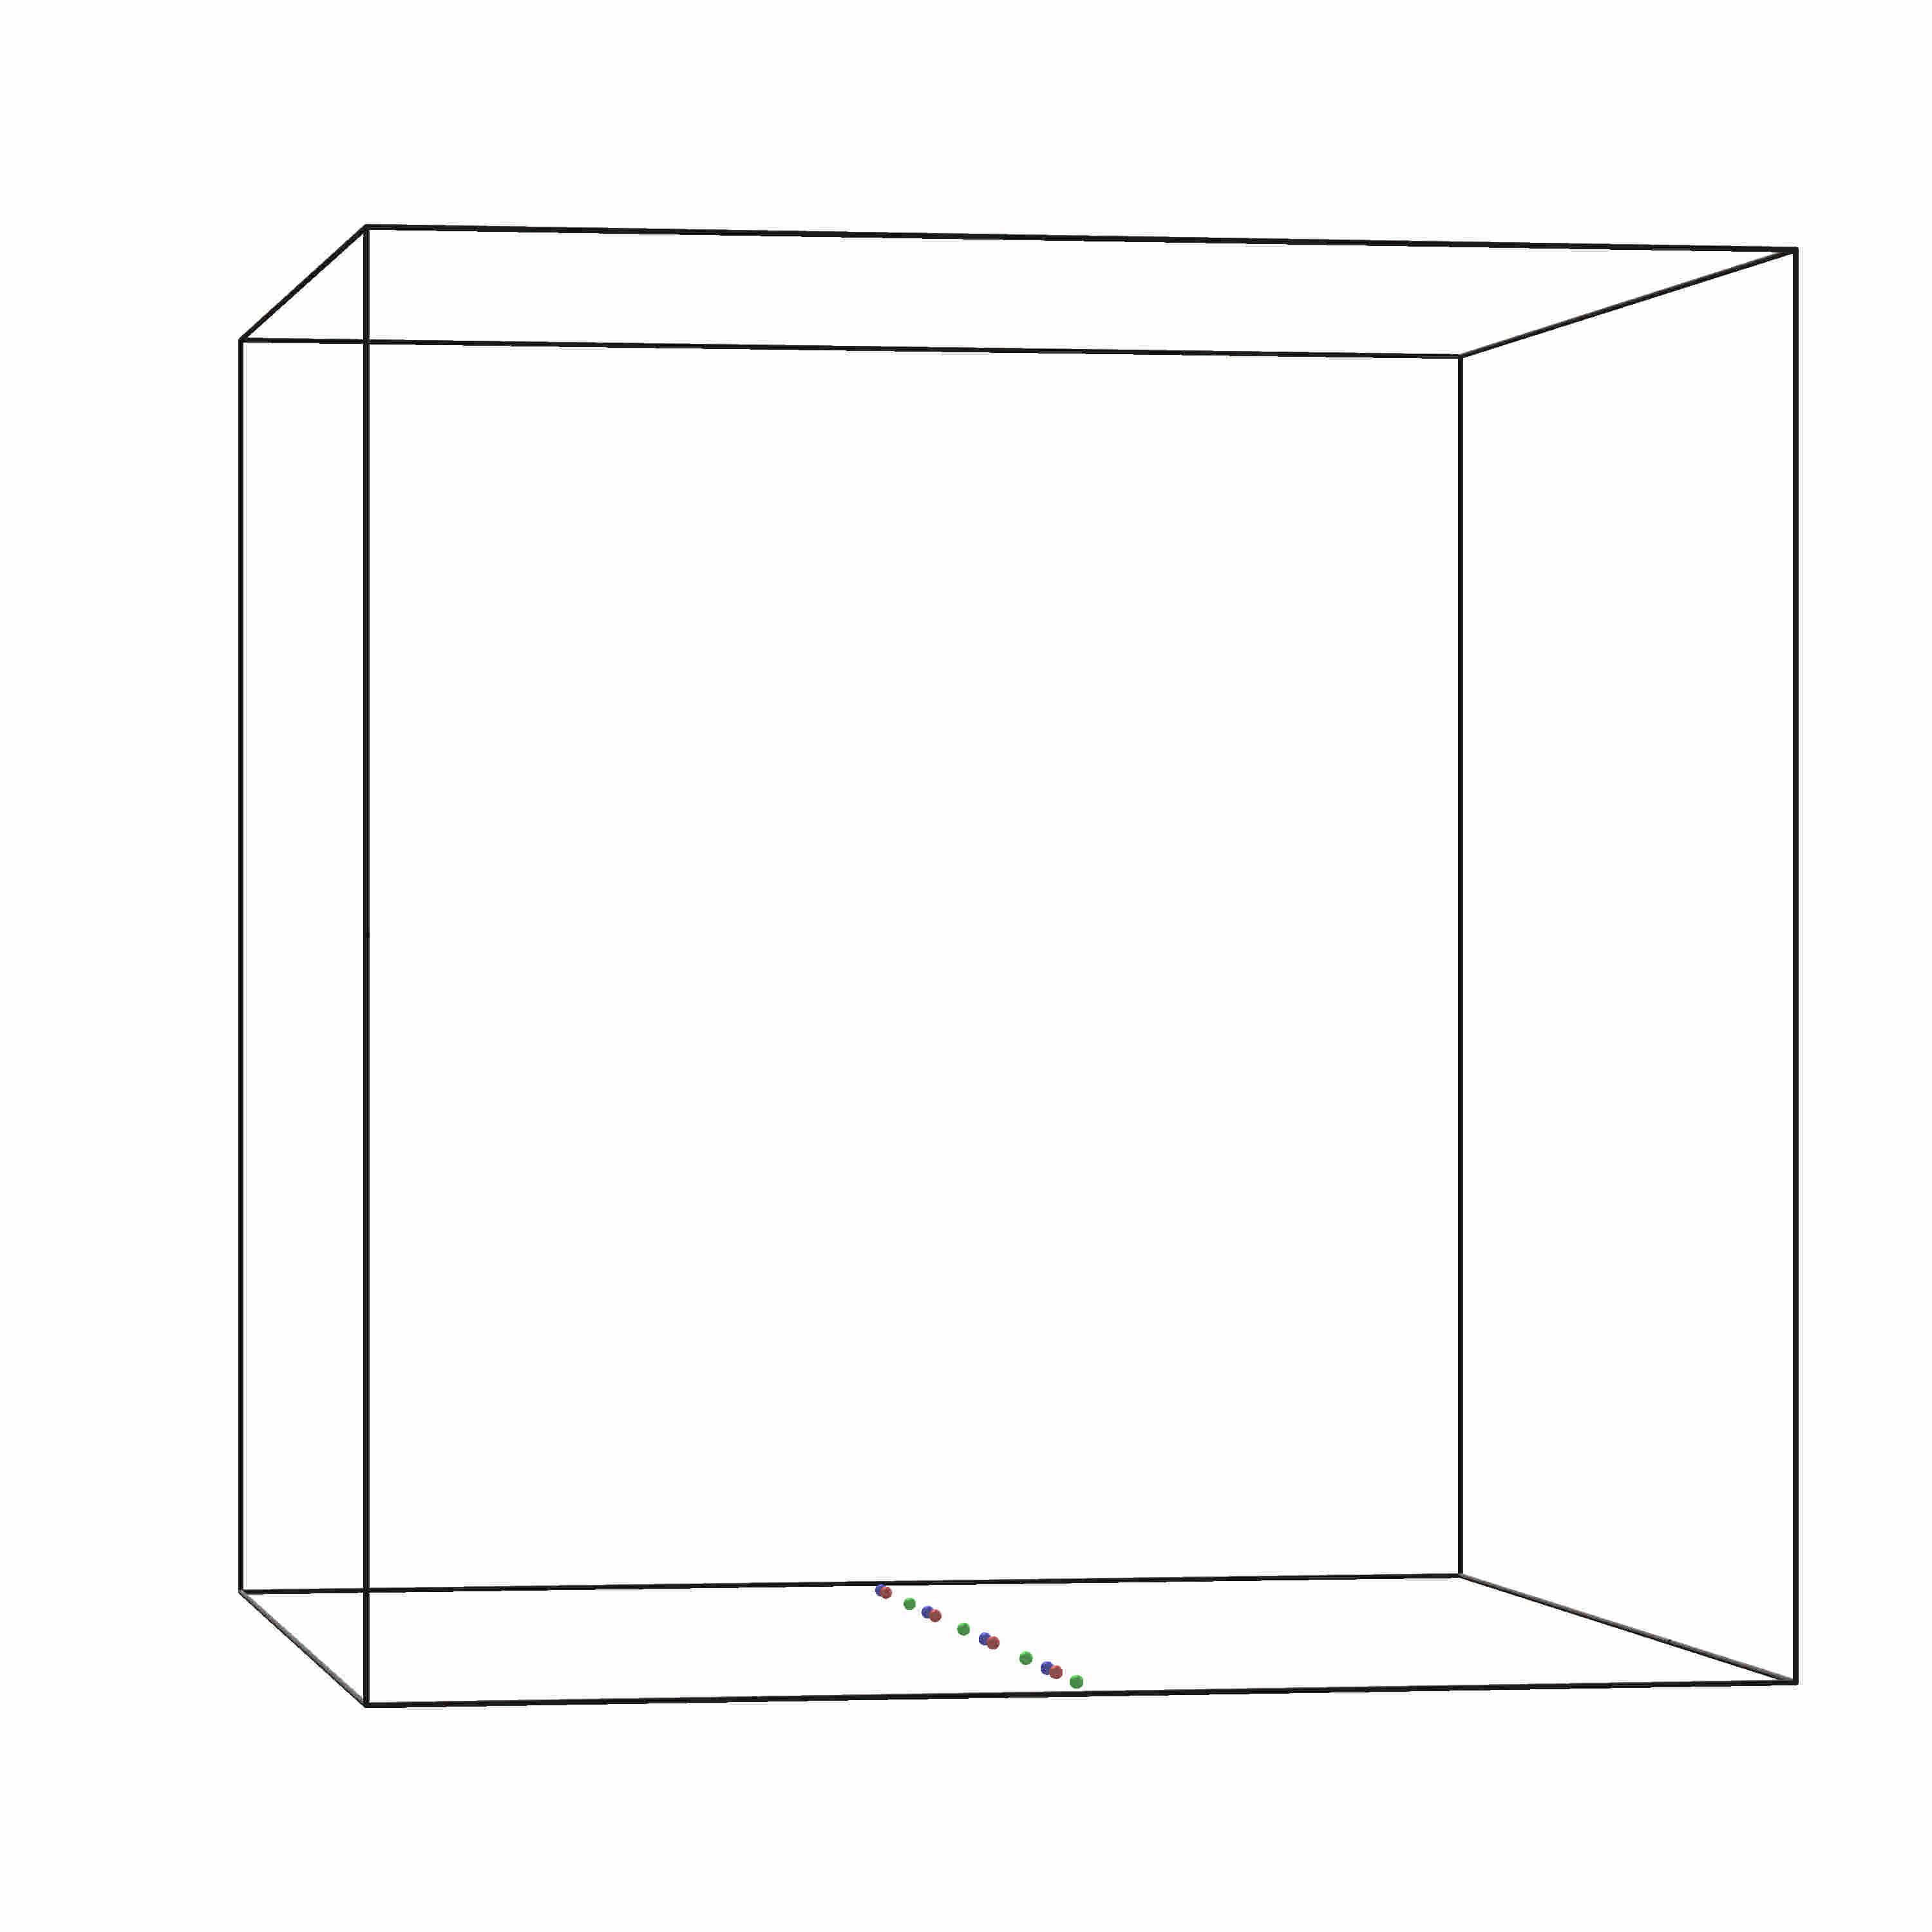
\includegraphics[height=.4\textheight]{image1000001}
\caption{time t=0)}
\label{}
\end{subfigure}%\vspace*{-.1em}
%\centering
\begin{subfigure}[b]{.5\textwidth}
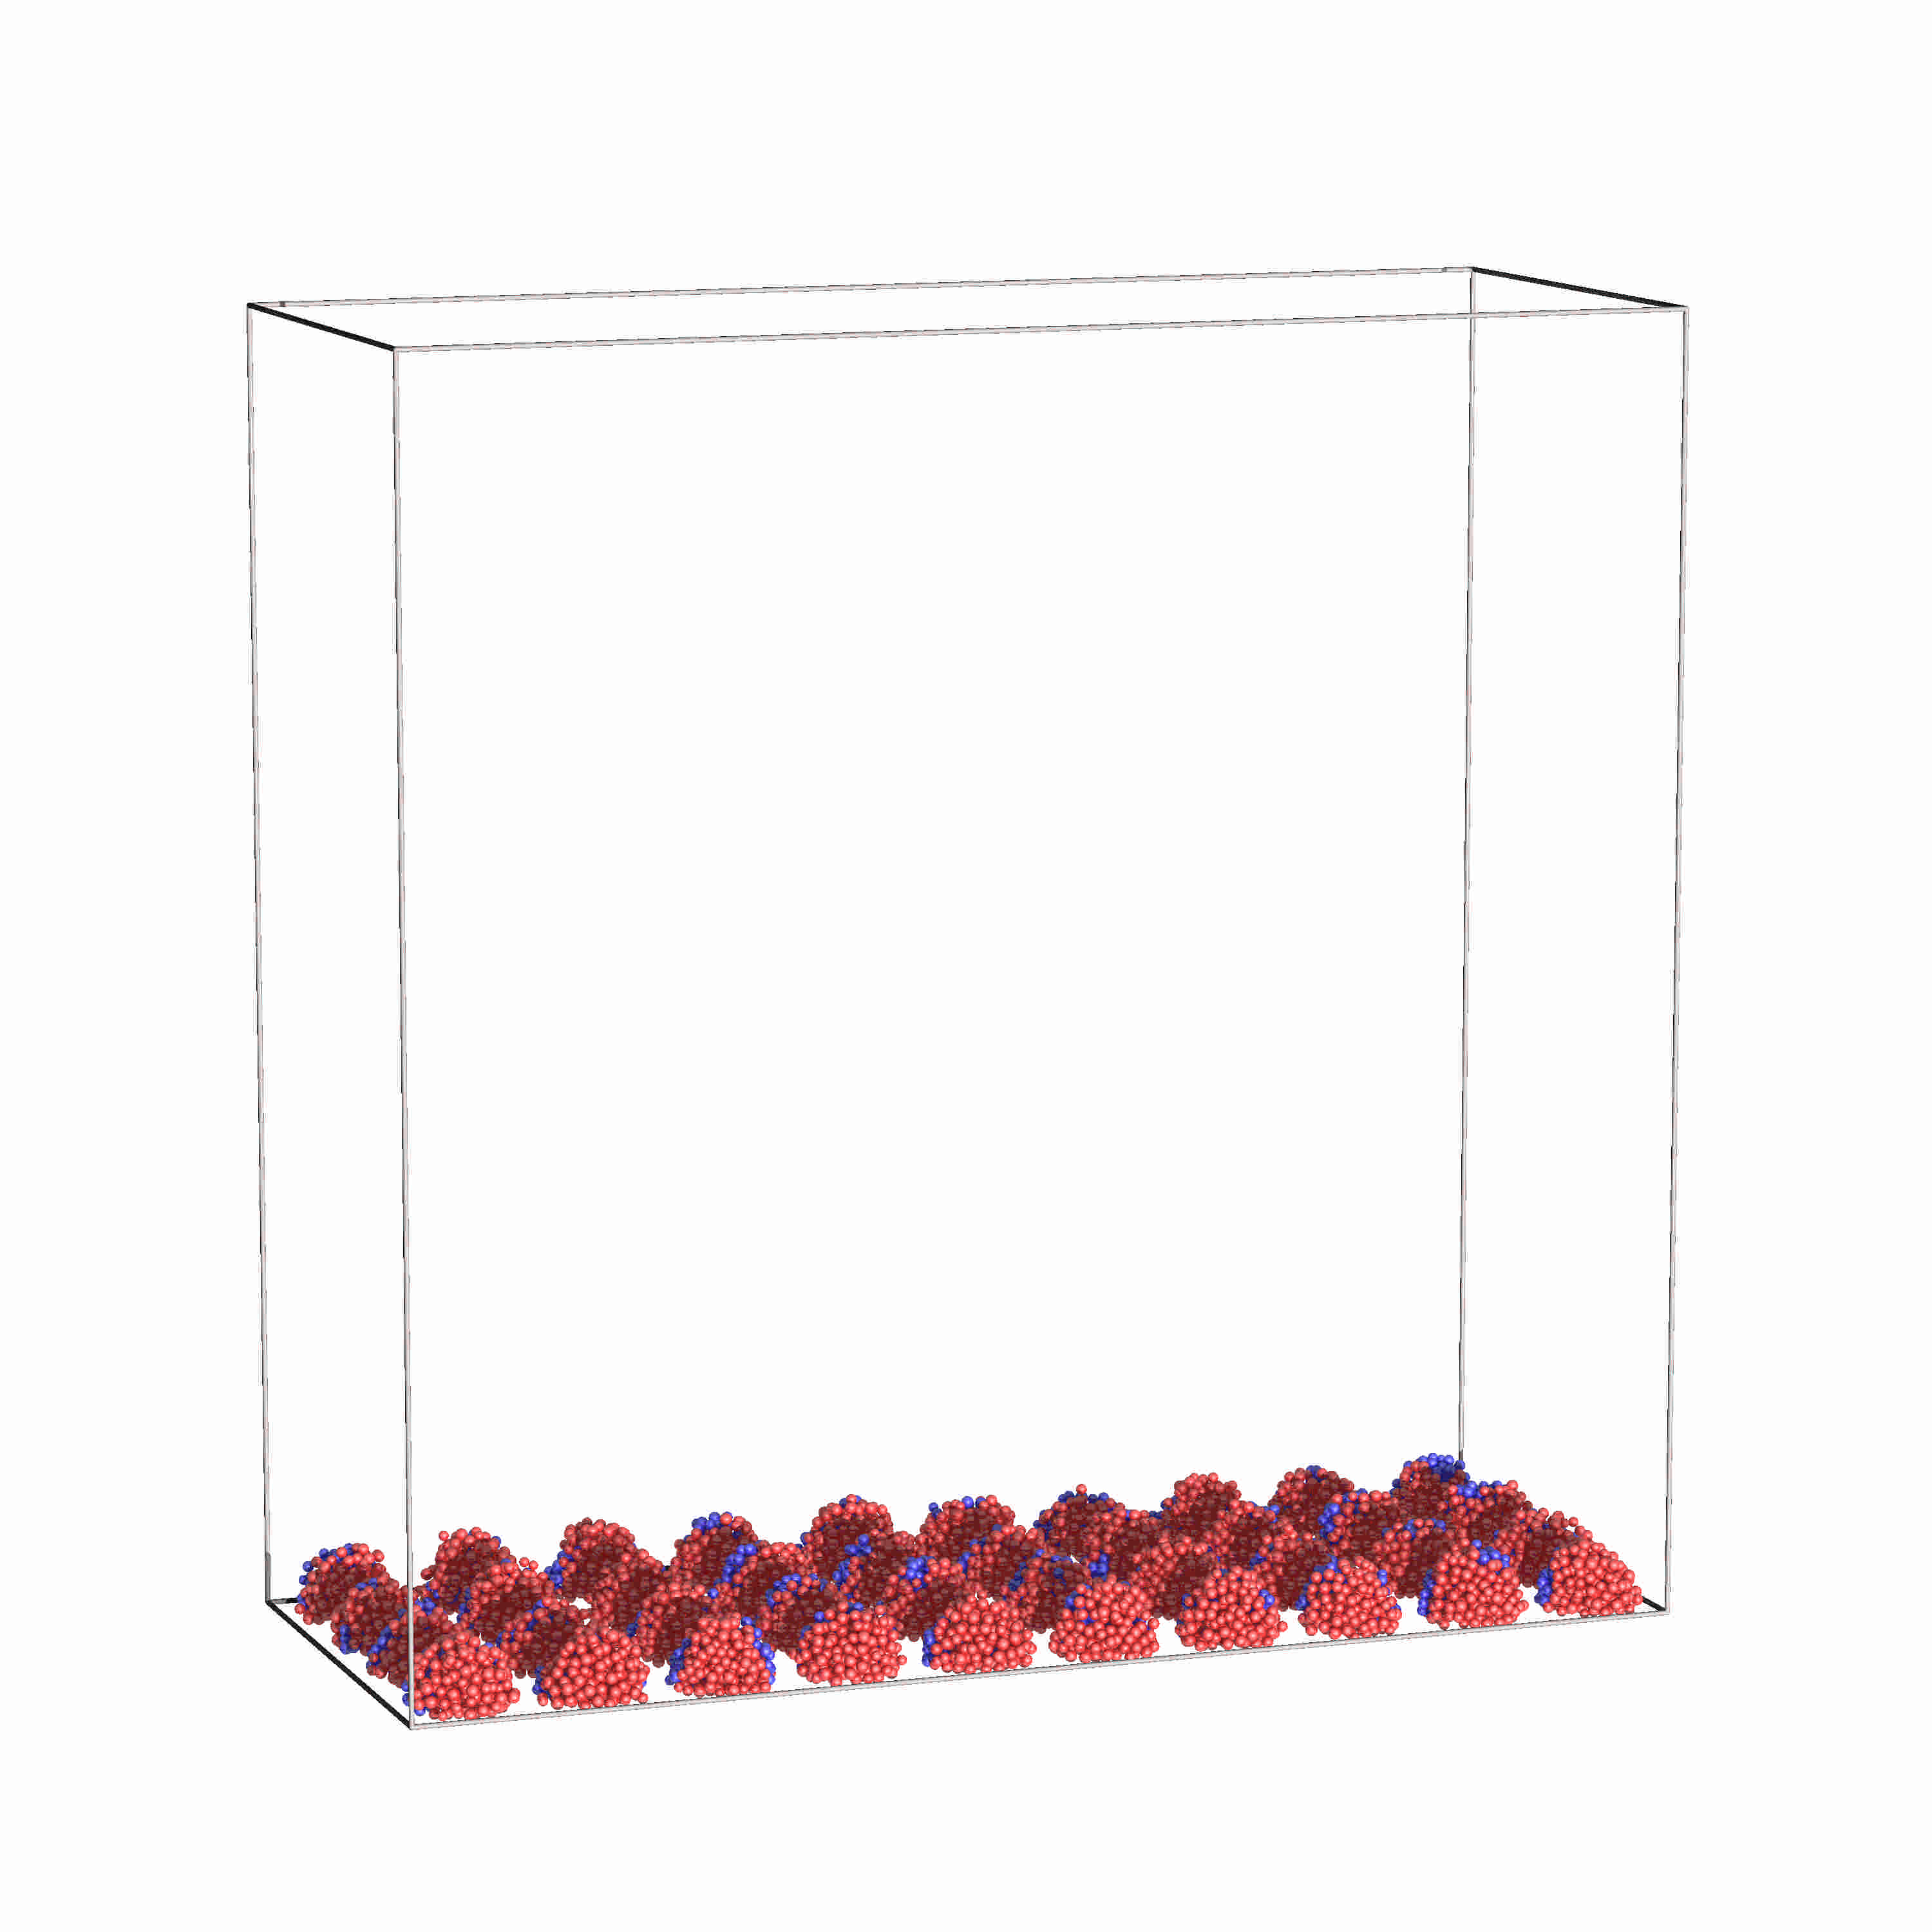
\includegraphics[height=.4\textheight]{image1000050}
\caption{time t=100000}
\label{}
\end{subfigure}\vspace*{-.1em}
% \centering
\begin{subfigure}[b]{.5\textwidth}
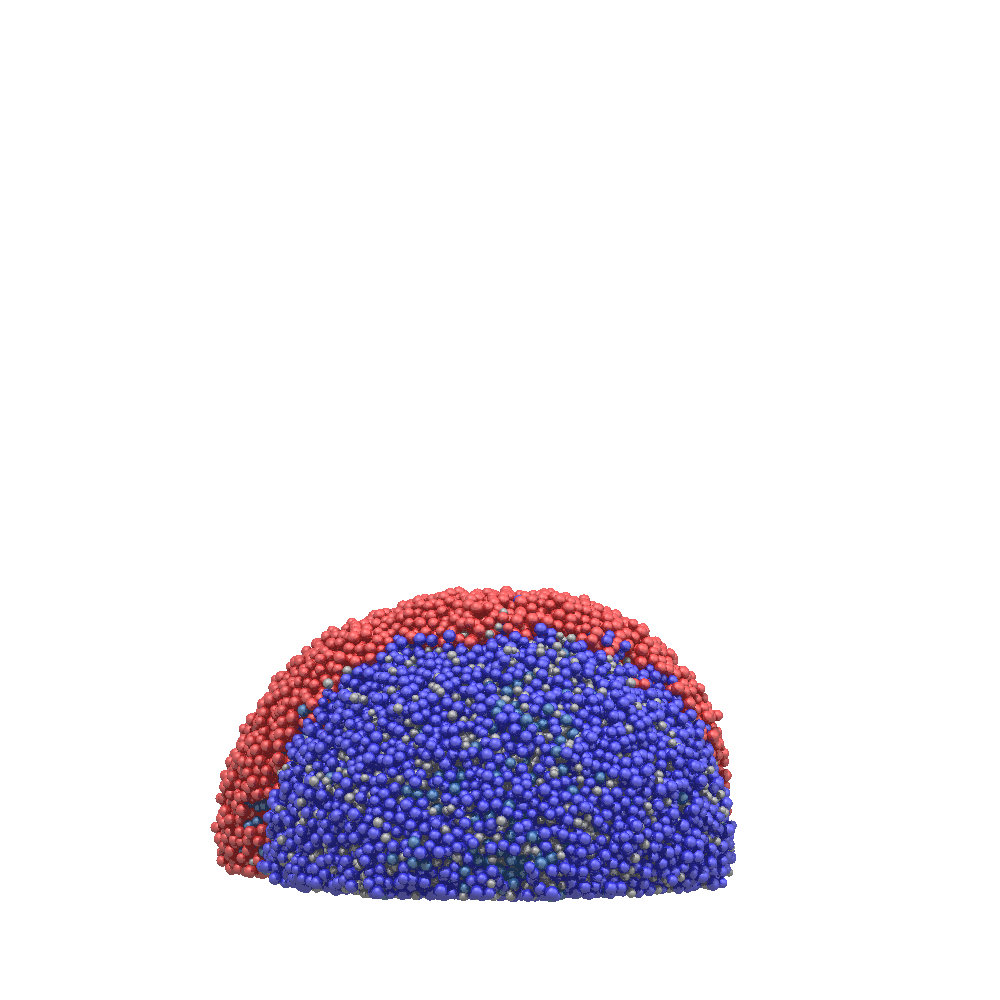
\includegraphics[height=.4\textheight]{image1000150}
\caption{time t=300000}
\label{}
\end{subfigure}\vspace*{-.1em}
%\centering
\begin{subfigure}[b]{.5\textwidth}
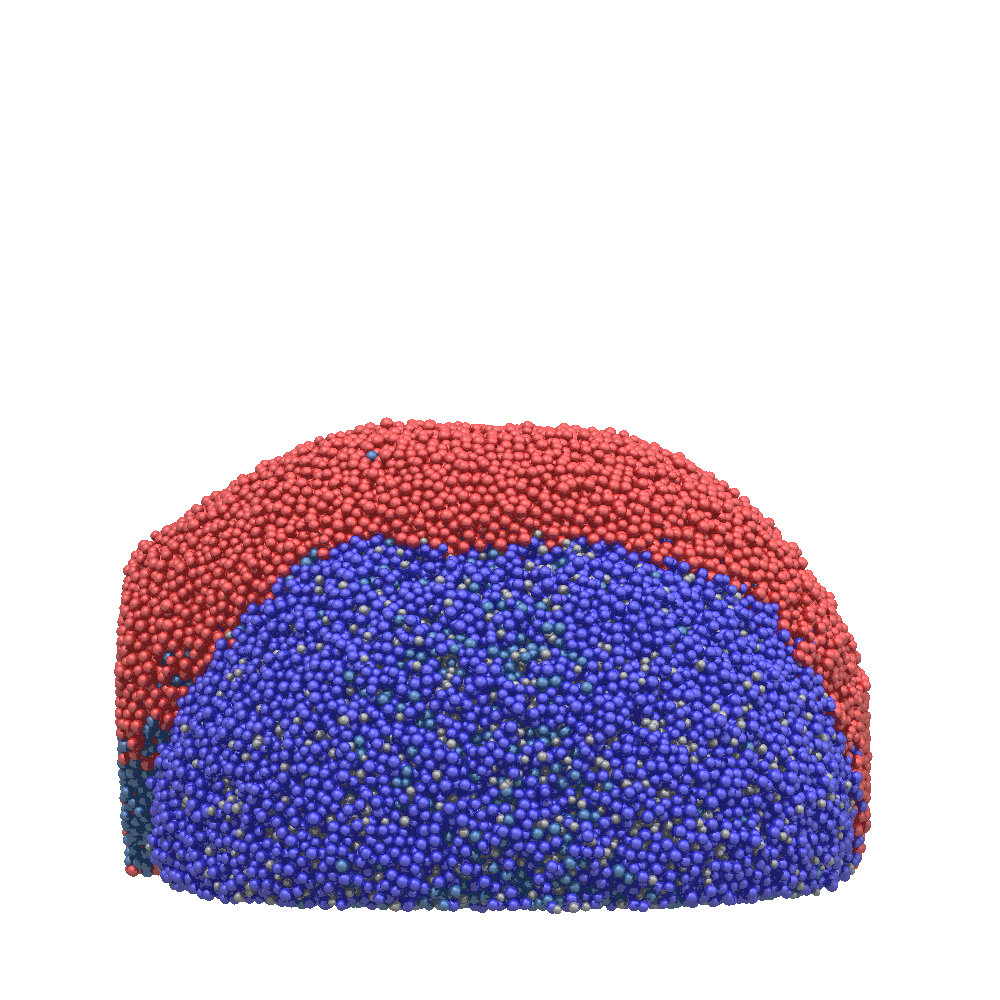
\includegraphics[height=.4\textheight]{image1000175}
\caption{time t=350,000}
\end{subfigure}\vspace*{-.1em}
\caption{Sample of LAMMPS simulation data for particle growth for 4 different time points (seconds).}\label{myfig1}
\end{figure}


\subsection{Simulation data}
We describe two different simulation procedures. Firstly, let the design matrix which contain the input to the LAMMPS model be denoted by $D=(\theta^i_p, t_p, p=1,\ldots,22; i=1,\ldots,100)$, where the subscript $p$ represents the 22 input parameters and superscript $i$ denote 100 different realisations (design points), $t_p$ is the time in seconds at which the output data is recorded. The design matrix $D_{100 \times 23}$ denotes the input values at which the LAMMPS model will be run for every combinations of $x_p$ where $x_p$ represents $p^{th}$ row of $D$. The current LAMMPS code is set up to produce the following outputs namely particle diameter, position (3-dimensional), velocity (3-dimensional) and force (3-dimensional). The LAMMPS code could be run for as long as there are sufficient computing resources to store the outputs. For the present analysis, the code is run for 352800 seconds to generate sufficient data for the emulation which is equivalent to $\approx$ 4 days of real time and generated output results are saved at a time-step of 2000 seconds which gives about 176 different time slices. 

Therefore, a single run of the code for each of design point $x_p$ will produce 10 different outputs and 176-time steps. There are five different types (or species) of the particle in the simulation namely AOB, NOB, HET, EPS and inert. We note that the shape and number of particles as well as the composition of the floc at each time step vary in the simulation. 

We perform the second simulation using the same input configuration as described above but repeated the runs for five times to incorporate stochastic variations in our outputs. This, of course, increases the amount of CPU time for the entire simulations even with running the bash script in parallel on a Linux machine. 


\section{Method 1: Combination of linear models and Gaussian process regression}
\subsection{Procedure}
We describe the analysis of the first data set here.
The work focuses on predictions of mean floc diameter from LAMMPS simulation outputs together with their associated uncertainty levels. We propose a two-stage approach similar to \citet{pd11} where we shall combine a linear model in the first stage and a Gaussian process regression for residual interpolation in the second stage.

The step by step procedure for emulating one of the outputs of LAMMPS model, "particle floc diameter" is given here. We start by computing the average diameter of all the particles at each time step to obtain a vector $\by(x)=\bar z_1,\ldots,\bar z_{176}$ of the mean floc diameter to be emulated such that
\begin{equation}
\bar z_t=\frac{\sum^N_{k=1} z_{kt}}{N}
\end{equation}
where $k=1,\ldots, N$, $N$ represents the total number of all 5 particles at each time slice. We also note that $N$ varies across time point and in particular increases with time as seen in Figure \ref{myfig1} and $z_{kt}$ is a simulation floc diameter for particle $k$ at time $t$.

\subsection{Stage 1: Linear models}
For the training data, we sub-sample 75 out of 176-time slices for each design point $x_p$ which gives a total of 7500 observations.
The training data are ($7500 \times 1$) vector of mean floc diameter $\by$ of LAMMPS output and ($7500 \times 23$) matrix $\bX$, which holds the values taken by the explanatory variables. (NOTE: sequence of time $t$ at which output is sought is used as an additional input to the emulator). We fit a linear model to data $[\by,\bX]$ and then obtain the predictions $\hby$.
We also use the fitted model to predict the left out observations $\tby^{new}$ for cross-validation purpose and to obtain standard error of predictions $\bs^{new}$, which is a measure of prediction uncertainty in the linear model. 

%Finally, we apply a GP to model the residual field obtaining from the linear model.
In order to construct emulator for the prediction of mean particle diameter, we apply a standard regression to the data in the first stage using equation (\ref{geneq}) and use a Gaussian process regression for interpolating unexplained residual from linear model
\begin{equation}\label{geneq}
\by=f(\textbf{\bx})+\boldsymbol\varepsilon= \beta'_0+\beta'_{1}x_{1}+\ldots +\beta'_{p}x_{p}+\boldsymbol\varepsilon
\end{equation}
where $\by$ is the LAMMPS simulated mean floc diameter, $p=23$ is the number of parameters for estimation and $\bx_1,\ldots,\bx_p$ are independent variables and $\beta'_1,\ldots,\beta'_{23}$ are regression coefficients. We assume $\boldsymbol \varepsilon \sim N(0, \sigma^2)$. 

\subsection{Summary of steps taken for stage 1 modelling}
\begin{itemize}
\item[{(i)}] Design of experiment to identify important outputs (which outputs are to be emulated). 
\item[{(ii)}] Determine the relevant input factors to be varied (use all the 22 factors for now). 
\item[{(iii)}] Assign uniform probability density to each input variable (we have little knowledge about these parameters). 
\item[{(iv)}] Generate LHS of 100 design points on each of the 22 input parameters and transform into the quantile of uniform distribution using parameter ranges in Table \ref{mytab1}. 
\item[{(v)}] Evaluate LAMMPS model for various input combinations to obtain the training data.
\item[{(vi)}] Compute the LAMMPS mean floc diameter for each time-step from output data
\item[{(vii)}] Randomly sample 75 time points out of 176 for each design point
\item[{(viii)}] Fit a linear model with equation (\ref{geneq}) using all 23 parameters (time is included as an additional variable to the linear model)
\item[{(ix)}] Obtain both predictions and standard error of predictions for all data points
\end{itemize}

\subsection{Stage 2: GP modelling of residual data}\label{GP}
The (${7500\times 1}$) vector of residual $\boldsymbol \varepsilon=\by-\hby$ obtained from stage 1 formed our new training data in this section. This residual can be modelled as $\boldsymbol \varepsilon= \eta(X')$. We do not apply GP to all the 23 input variables in stage 1. Rather, we use standardized regression coefficients of equation (\ref{geneq}) as a measure of sensitivity to select important explanatory variables for the GP regression such that $X'<< X$ (ie $p$ is now $<23$).
Since Gaussian process is described completely by its mean and covariance functions, the mean function is given as
\begin{equation}\label{eqgp3}
E[\eta(X')|\boldsymbol\beta]=h^{\rm T}(\bX')\boldsymbol\beta,
\end{equation}
where $h(\bX')$ is a vector of regression functions. For our analysis, we use a simple linear function $h(\bX') = (1,\bx^T$) and $\boldsymbol\beta$ is an unknown hyperparameter to be estimated and covariance function $$ K={Cov[\eta(\bx),\eta(\bx')|\sigma^{2},\boldsymbol \alpha]=\sigma^{2} \bC(\bx,\bx^{\rm T})},$$ where $\sigma^{2}$ is a noise variance and $\bC(\bx,\bx^{\rm T})$ is a correlation function with an hyperparameter $\boldsymbol \alpha$. Gaussian and exponential correlation functions of the form
\begin{equation}\label{gaus}
\bC=\Big \{\exp(-(x-x')^T \boldsymbol \alpha (x-x')) \Big\},%\exp^{\Big[\sum \limits_{j=1}^{4}{-\boldsymbol \alpha_j(\bx_{j}-\bx^{\rm T}_{j})^2}\Big]}.
\end{equation}
\begin{equation}\label{expo}
\bC= \exp(-(x-x')/\alpha)
\end{equation}
where $\boldsymbol \alpha$ is the correlation hyperparameters to be estimated from the data. It is difficult to apply a GP directly to the entire residual data because of the inversion of covariance matrix which scales cubically with the number of
observations O($N^3$), we proceed by sub-sampling just 200 random observations from the data and denote the training data as $[\by, \bX']$, where $\by=[ \varepsilon_1= \eta(x_1),\ldots, \varepsilon_{200}= \eta(x_{200})]$. We select just 4 important explanatory variables for the GP modelling and our correlation parameter is denoted as $\boldsymbol \alpha=(\alpha_1,\ldots,\alpha_4)$.

For computing the posterior distribution, we assign a non-informative prior to the $\boldsymbol \beta$, $\sigma^2$ and $\alpha$ parameters such that $p(\bbeta, \sigma^2) \sim \sigma^{-2}$ and $p(\alpha) \sim 1$.
We update these prior distributions on some data $\by$ to get the posterior estimates using Bayes theorem. We estimate their values by conditioning on each parameter and maximize the resulting marginal likelihood function \citep{pd7,pd10}. Therefore, the resulting posterior distribution is denoted as $\eta(.)|\by \sim N\Big \{\mu^{\star}, K^{\star} \Big\}$, where

\begin{equation}\label{olu1}%\tag{A.8}\label{olu1}
\mu^{\star}(\mathbf{x})=h(\mathbf{x})^T\boldsymbol{\hat\beta}+t(\mathbf{x})^T\bC^{-1}[\by-\bH\boldsymbol{\hat\beta}]
\end{equation}
\begin{multline}\label{olu2}%\tag{A.9}\label{olu2}
\begin{split}
K^{\star}=\hat \sigma^2 \Big \{c(\mathbf{x,x'}) -t(\mathbf{x})^T\bC^{-1} t(\mathbf{x}) + \\ \Big ( h(\mathbf{x})^T-t(\mathbf{x})^T\bC^{-1}t(\mathbf{x}) \Big )
(\bH^T\bC^{-1}\bH)^{-1}\Big ( h(\mathbf{x'})^T-t(\mathbf{x'})^T\bC^{-1}t(\mathbf{x'}) \Big )^T
\Big \}
\end{split}
\end{multline}
where $t(\bx)^T=[c(\bx,\bx_1),\ldots, c(\bx,\bx_n)]$ and $\bH^T=[h(\bx_1),\ldots, h(\bx_n)]$, see more details in the appendix. We analyse our results using $emulator$ package in $R$.

Finally, let the GP posterior mean and variance estimates of the residual at a new input point $x^{new}$ (cross-validation) be denoted as $\mu^{\star \star}$ and $K^{\star \star}$ respectively, and predictions and standard error of predictions from linear model as $\tby^{new}$ and $\bs^{new}$ respectively. The final predictions of mean particle diameter $\hby^{new}$ is given as
\begin{equation}\label{r1}
\hby^{new} = \tby^{new} +\mu^{\star \star}(\bx)
\end{equation}
and total uncertainty is
\begin{equation}\label{r1}
\hat \bs^{new} = \bs +\sqrt{|K^{\star \star}}|
\end{equation}

\subsection{Summary of stage 2}
\begin{itemize}
\item[{(i)}] Perform the GP emulation of the unexplained residual data 
\item[{(ii)}] Given the posterior density of $\alpha$ as defined in equation (\ref{like3}) of Appendix 1, compute the MLE of $\balpha$, such that equation (\ref{like3}) is maximized.
\item[{(iii)}] Set $\bC= \bC(\bhalpha)$
\item[{(iv)}] Compute estimate $\hbbeta=(\bH^T\bC^{-1}\bH)^{-1}\bH^T\bC^{-1}\by$
\item[{(v)}] Compute estimate $\widehat{\sigma^2}=\frac{1}{n-p}\Big[\mathbf{(y-H\hat{\boldsymbol \beta})}^T\bf C^{-1}(\bf y-H\hat{\boldsymbol \beta})\Big]$
\item[{(vi)}] Compute posterior mean estimate $\mu^{\star}(\mathbf{x})$ given in equation (\ref{olu1})
\item[{(vii)}] Compute posterior variance estimate $K^{\star}$ given in equation (\ref{olu2}) above
\end{itemize}

\begin{figure}[!ht]
\begin{subfigure}[b]{.5\textwidth}
%\centering
\includegraphics[height=10cm,width=1.1\textwidth]{res_plots/wole1}
\caption{LAMMPS and model predictions (emulator) for some randomly selected points}
\label{myfigg9a1}
\end{subfigure}\hspace*{1em}
\begin{subfigure}[b]{.5\textwidth}
%\centering
\includegraphics[height=10cm,width=1.1\textwidth]{res_plots/wole2}
\caption{LAMMPS and model predictions (emulator) for some randomly selected points}
\label{myfigg9a1}
\end{subfigure}
\begin{subfigure}[b]{.5\textwidth}
%\centering
\includegraphics[height=10cm,width=1.1\textwidth]{res_plots/wole3}
\caption{LAMMPS and model predictions at $79^{th}$ design point for all time steps}
\label{myfigg9a1}
\end{subfigure}\hspace*{1em}
\begin{subfigure}[b]{.5\textwidth}
%\centering
\includegraphics[height=10cm,width=1.1\textwidth]{res_plots/wole4}
\caption{LAMMPS and model predictions at $28^{th}$ design point for all time steps}
\label{myfigg9a2}
\end{subfigure}
\caption{Pair plot of model predictions (emulator) vs. LAMMPS values with their 95\% C.I for mean floc diameter (all species) from a two-stage technique}\label{myfig2}
\end{figure}


\chapter{Method 2: Kriging}
Having obtained the simulation data by running the LAMMPS model as described in the previous section, we describe an alternative emulation approach for fitting LAMMPS output data. This approach involves using a kriging model, where the two stage techniques describe in previous section are combined as a single step. Kriging is a geostatistical technique for interpolating the value of an unknown random observation from data $\by(\bx)$ observed at known locations. Kriging models are also commonly used for building cheaper surrogate model of expensive computer codes \cite{pd1,pd2, pd3,pd6}. Here, $\by(\bx)$ can be decomposed into a mixture of deterministic (non-random trend) and a residual random variation. The trend could be modelled as a constant in ordinary/simple kriging or as an $n^{th}$ order polynomial in universal kriging. In this section, we shall discuss the universal kriging technique. The model formulation is given as
\begin{equation}\label{geneq2}
\by(\bx)= f(\bx) + \boldsymbol \varepsilon(\bx)
\end{equation}
where $\by(\bx)$ is as defined in equation (\ref{geneq}) above. The deterministic function $f(\bx)$ is the mean approximation of the expensive computer simulator (eg LAMMPS) and $f$ is a polynomial function. Under this assumption, $f(x)$ can be modelled as
\begin{equation}
f(\bx) = \sum_{j=1}^{p} \beta_j h_j(x) =\bH(x) \bbeta
\end{equation}
$\bbeta=[\beta_1,\ldots,\beta_p]$ is a $(p\times 1)$ vector of unknown regression coefficients and $\bH(x) = [h_1(x), . . . , h_p(x)]^T$ is a $(n\times p)$ matrix of regression functions,
$\varepsilon(\bx)$ is a stochastic Gaussian process with mean zero and characterize by its covariance function
$K=Cov(\varepsilon(\bx),\varepsilon(\bx)) = \sigma^2\bC(\bx,\bx')$, where $\sigma^2$ denotes the variance of $\varepsilon(\bx)$ also called process variance and $\bC$ is a $(n\times n)$ positive definite matrix of correlation between $\varepsilon(\bx)$'s at the experimental design points. We are assuming a univariate output and a deterministic computer model.
Similarly, $\bt(x^{new}) = [Cor(x_1, x^{new}), \ldots,Cor(x_n, x^{new})]^T$ for the $(n\times 1)$ vector of correlations between the $\varepsilon(\bx)$'s at the design points and new input points $x^{new}$. We use both Gaussian equation and exponential correlation functions, equations (\ref{gaus},\ref{expo}) \citet{pd4,pd18,pd19}.
%\begin{equation}
%\bC(x,x')=\Pi^{p}_{j=1}\exp^{-\balpha(x-x')^2}, 
%\end{equation}
%with a parameter $\balpha$. 

The universal kriging predictor $\hby^(x^{new})$ of the value of $\by(x)$ at the new target point $x^{new}$ is the linear predictor
\begin{equation}
\hby(x^{new})=\sum_{j=1}^n \lambda_j \by (x_j)=\lambda(x)^T\by,
\end{equation}
for the sample points $x_1, \ldots , x_n$, where the coefficients or weights $\lambda=(\lambda_1, \ldots, \lambda_n)^T$ are estimated by minimizing the variance of prediction error for each realizations of the random function $\by(x)$. The best linear unbiased predictor (BLUP) is computed by minimizing the mean squared error
\begin{equation}\label{mse}
MSE[\hby(x^{new})]=E[\lambda^T\by-\by(x^{new})]^2,
\end{equation}
subject to the unbiasedness constraint $E[\lambda^T(x)\by] = E[\by(x^{new})]$. The mean squared error in equation (\ref{mse}) can be rewritten by substituting the value of $\by$ in equation (\ref{geneq2}), we thus have 
\begin{equation}
\sigma^2[1 + c\lambda^T(x)\bC\lambda(x) - 2\lambda^T(x)\bt(x^{new})],
\end{equation}
The unbiasedness constraint is now denoted as $H^T\lambda(x) = h(x)$. 
The optimal weights $\lambda^{*}_j$ in $\by(x^{new})$ is estimated by using Lagrange multipliers to constraining MSE minimization. The Lagrange multiplier is also use to solve system of equations in order to compute $p$ coefficients of $\lambda$.
Given the inverse of matrix $\bC$, then the best linear unbiased predictor for kriging model is given as
\begin{equation}\label{man}
\hby_{uk}(x) = h^T(x)\hbbeta+ \bt^T(x)\bC^{-1}(\by -\bH\hbbeta)
\end{equation}
Similarly, the variance follows by substituting in the optimal value of $\lambda^*(x)$ in the MSE equation, we have
\begin{multline}\label{olu2b}%\tag{A.9}\label{olu2}
\begin{split}
\hat S^2_{uk}=\hat \sigma^2 \Big \{C(\bx,\bx') -\bt(\bx)^T\bC^{-1} \bt(\bx) + \\ \Big ( h(\bx)^T-\bt(\bx)^T\bC^{-1}\bt(\bx) \Big )
(\bH^T\bC^{-1}\bH)^{-1}\Big (h(\bx')^T-\bt(\bx')^T\bC^{-1}\bt(\bx') \Big )^T
\Big \}.
\end{split}
\end{multline}
See more details in \citep{pd4,pd5,pd20}
%where $\hbbeta$ is given below.%= (\bH^T\bC^{-1}\bH)^{-1}\bH^T\bC^{-1}\by$.

The next problem is how to estimate the unknown parameters. We use a Maximum Likelihood Estimation (MLE) technique like many other authors \citep{ pd5,pd28}, as an objective estimator of the kriging model parameters because of its computational efficiency, $\theta=(\bbeta,\sigma^2,\boldmath \alpha)$. MLE assumes a Gaussian probability distribution. 
The likelihood of the model parameters is defined as the probability of the $n$ observations $\by= {y_1, …, y_n}$, given the model parameters such that 
\begin{equation}
L(\theta|\by)= \Pi_{j=1}^n p(\by_j|\theta).
\end{equation}
The expression for $L(\theta|\by)$ is given by equation below as
\begin{equation}\label{like*}
L(\boldsymbol \beta, \sigma^2, \boldsymbol{\alpha};\by)\propto \frac{|\bf C|)^{-\frac{1}{2}}}{{(2\pi\sigma^2)}^\frac{n}{2}}\exp \Big \{\frac{(\by-H\boldsymbol \beta)^T \bf C^{-1}(\by-H\boldsymbol \beta)}{2\sigma^2}\Big\}
\end{equation}
where $\boldsymbol{\alpha}=[\alpha_1, \ldots, \alpha_n]$ is a vector of correlation lengths and $|\bC|$ is the determinant of correlation matrix $\bC$ and $K = \sigma^2\bC$.
By taking the derivative of the log-likelihood of equation (\ref{like*}) with
respect to $\bbeta$ and $\sigma^2$ and solving for zero, the estimates $\hbbeta$ and $\hat\sigma^2$ are given respectively as $\hbbeta=(\bH^T\bC^{-1}\bH)^{-1}\bH^T\bC^{-1}\by$ and $\hat{\sigma^2}=\frac{1}{n}\Big[\mathbf{(y-H\hat{\boldsymbol \beta})}^T\bf C^{-1}(\bf y-H\hat{\boldsymbol \beta})\Big]$. In order to estimate $\balpha$, we maximize over $\balpha$ the concentrated likelihood given below after plugging the values of $\hbbeta$ and $\hat\sigma^2$
\begin{equation}
-2 log L(\hbbeta, \hat \sigma^2, \balpha; \by) = n log(2\pi) + n log\hat \sigma^2 + log(|\bC|) + n
\end{equation}
The trend and covariance parameters $\theta$ are computed quickly and very efficiently by using a global optimiser which is based on the extension of efficient algorithm proposed in \cite{pd9} for likelihood maximization. See further details in \citep{pd8}.

For the noisy observations, covariance $K=\sigma^2\bC$ is replaced by $ \sigma^2\bC+\btau^2$I in equations (\ref{like*},\ref{olu2b},\ref{man}) respectively, where $\btau^2=\tau^2_1,\ldots,\tau^2_n$ are the noise variances and $I$ is a diagonal matrix of ones. Kriging technique is equivalent to the Bayesian method describes in section (\ref{GP}) if we assign improper uniform priors on the $\bbeta$. In other words, non-informative Bayesian analysis often leads to kriging predictor and variance and these estimators appear respectively as conditional mean and variance in equations (\ref{olu1} and \ref{olu2}).


\section{Kriging results}
Some results from kriging technique are given here. Recall from above that our training data are ($7500 \times 1$) vector of mean floc diameter $\by$ of LAMMPS output and ($7500 \times 23$) matrix $\bX$ of input variables. Here, we use the same 75 out of 176-time slices but we sub-sample just 50 design points to further reduce the dimension of the data which gives a total of 3750 observations. The new training data for the kriging model is $D=[\by_{3750 \times 1}, X_{3750 \times 23}]$. We consider only the linear terms for the trend model (no quadratic terms). We compare both Gaussian and exponential covariance functions with little difference in their predictions. The performance of the kriging emulator is tested by using the fitted model to predict the left out data. 

We also perform the sensitivity analysis of the mean particle floc diameter to identify relevant variables. We use a Sobol technique which involves decomposing total output variance as a summand of increasing dimensionality. We sampled 1000 observations from a uniform distribution for each of the 23 input variables in Table 1. We compute the sensitivity indices for three different methods. Bootstrapping was used to compute 95\% confidence intervals on the estimated indices. The indices are shown in Figure \ref{sens} and we can see that only four parameters are relevant. Finally, we refitted the kriging model using just these four important parameters, some visual plots of results comparing the LAMMPS simulations with the emulator are showing in Figure \ref{myfig3}. We also compute the total percentage of variance explained by the final model which is $\sim 99\%$.



\begin{figure}[!ht]
\begin{subfigure}[b]{.5\textwidth}
%\centering
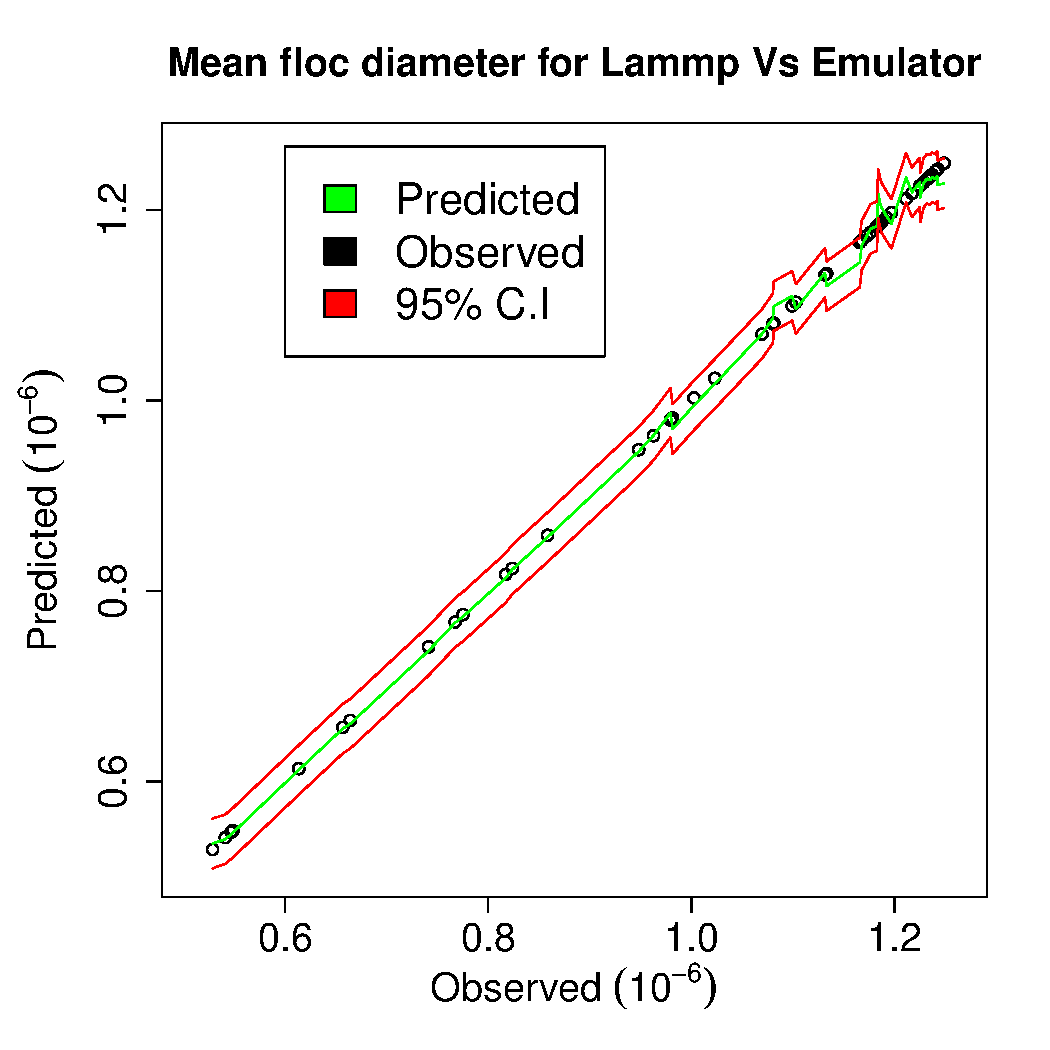
\includegraphics[height=9cm,width=1.1\textwidth]{ana/myplot1}
\caption{LAMMPS and kriging predictions (emulator) for some randomly selected points}
\label{myfigg9a1}
\end{subfigure}\hspace*{1em}
\begin{subfigure}[b]{.5\textwidth}
%\centering
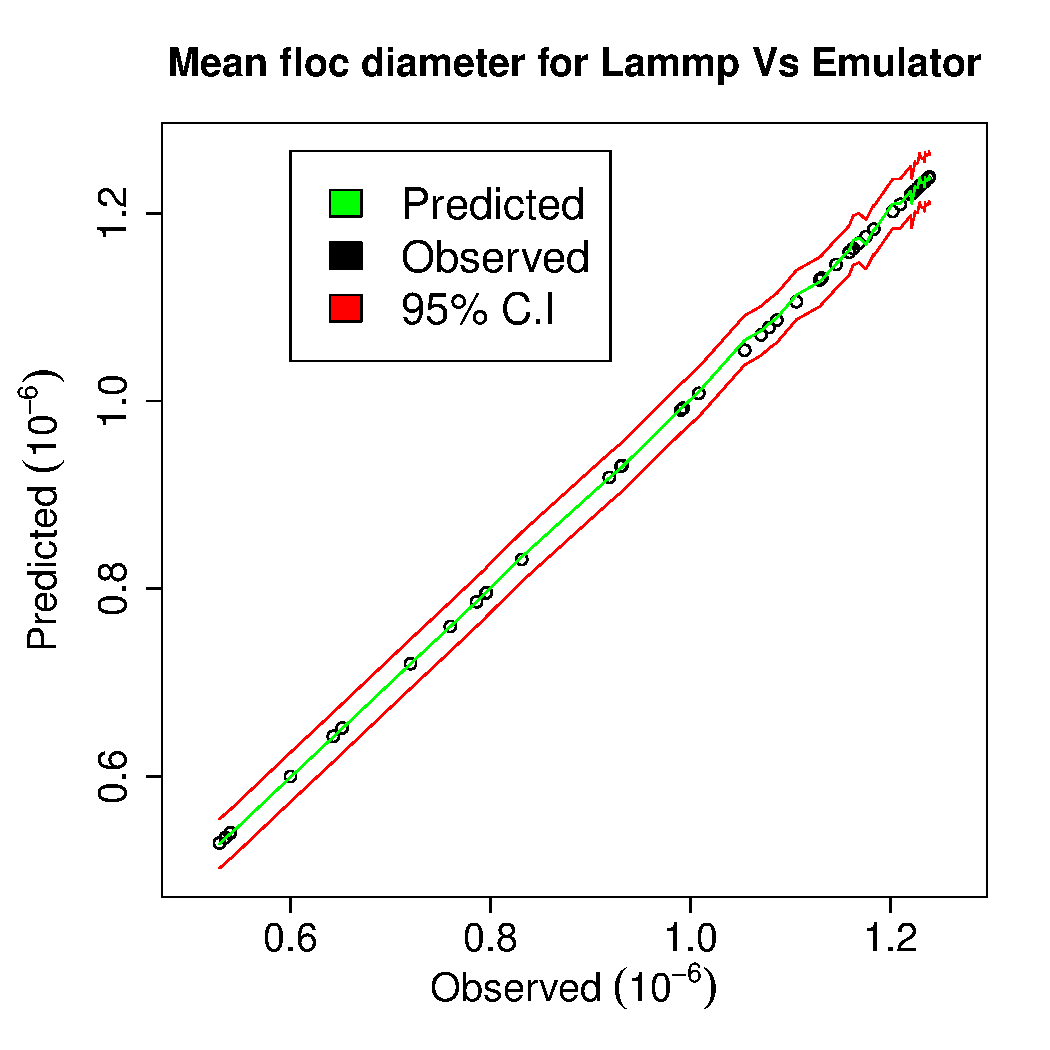
\includegraphics[height=9cm,width=1.1\textwidth]{ana/myplot2}
\caption{LAMMPS and kriging predictions (emulator) for some randomly selected points}
\label{myfigg9a1}
\end{subfigure}
\begin{subfigure}[b]{.5\textwidth}
%\centering
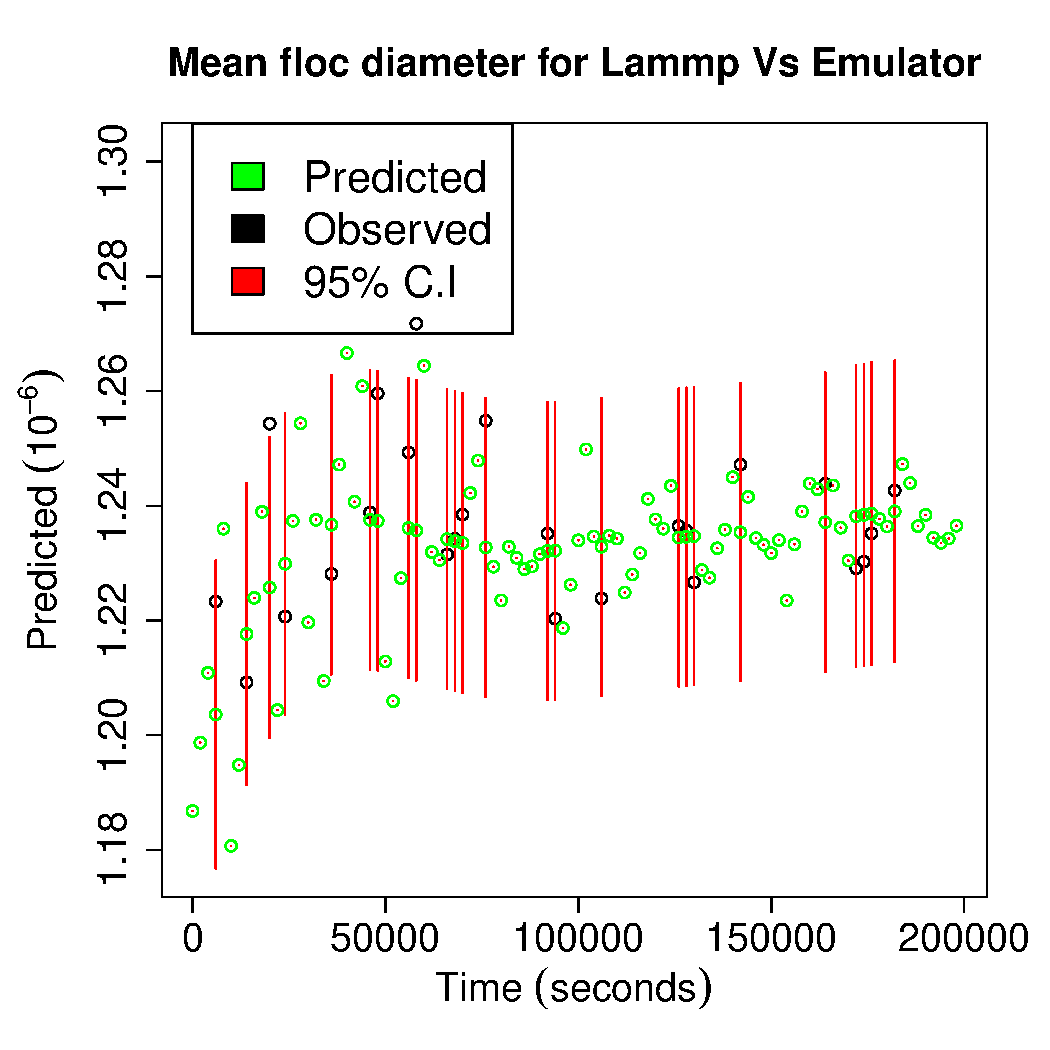
\includegraphics[height=9cm,width=1.1\textwidth]{ana/myplot5}
\caption{LAMMPS and kriging predictions at $20^{th}$ design point for all time steps. Note: The points with no C.I bands are the design points where MSE=0}
\label{myfigg9a1}
\end{subfigure}\hspace*{1em}
\begin{subfigure}[b]{.5\textwidth}
%\centering
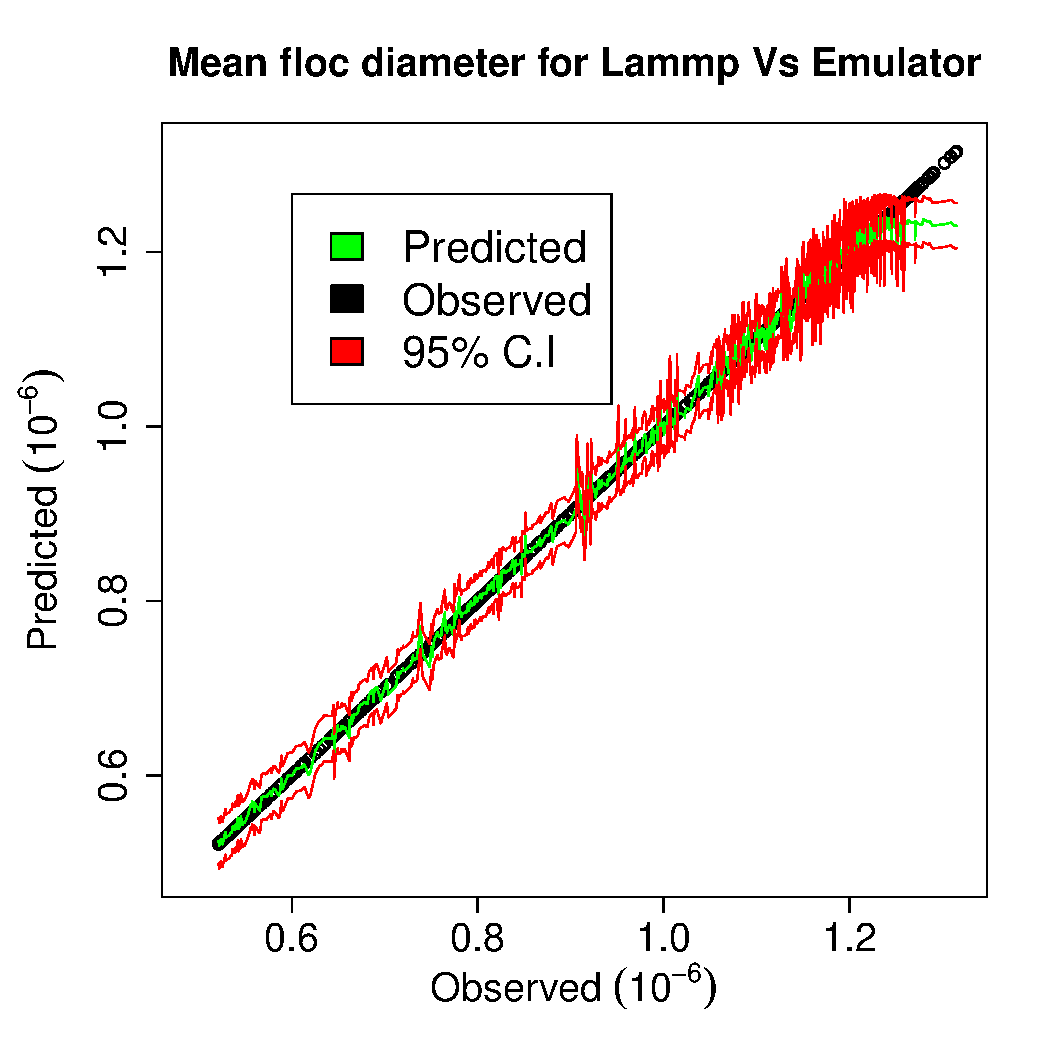
\includegraphics[height=9cm,width=1.1\textwidth]{ana/myplot3}
\caption{Pair plot for complete data set}
\label{myfigg9a2}
\end{subfigure}
\caption{Pair plot of kriging predictions (emulator) vs. LAMMPS values with their 95\% C.I for mean floc diameter (all species) using a Gaussian covariance functions}\label{myfig3}
\end{figure}

\begin{figure}[!ht] 
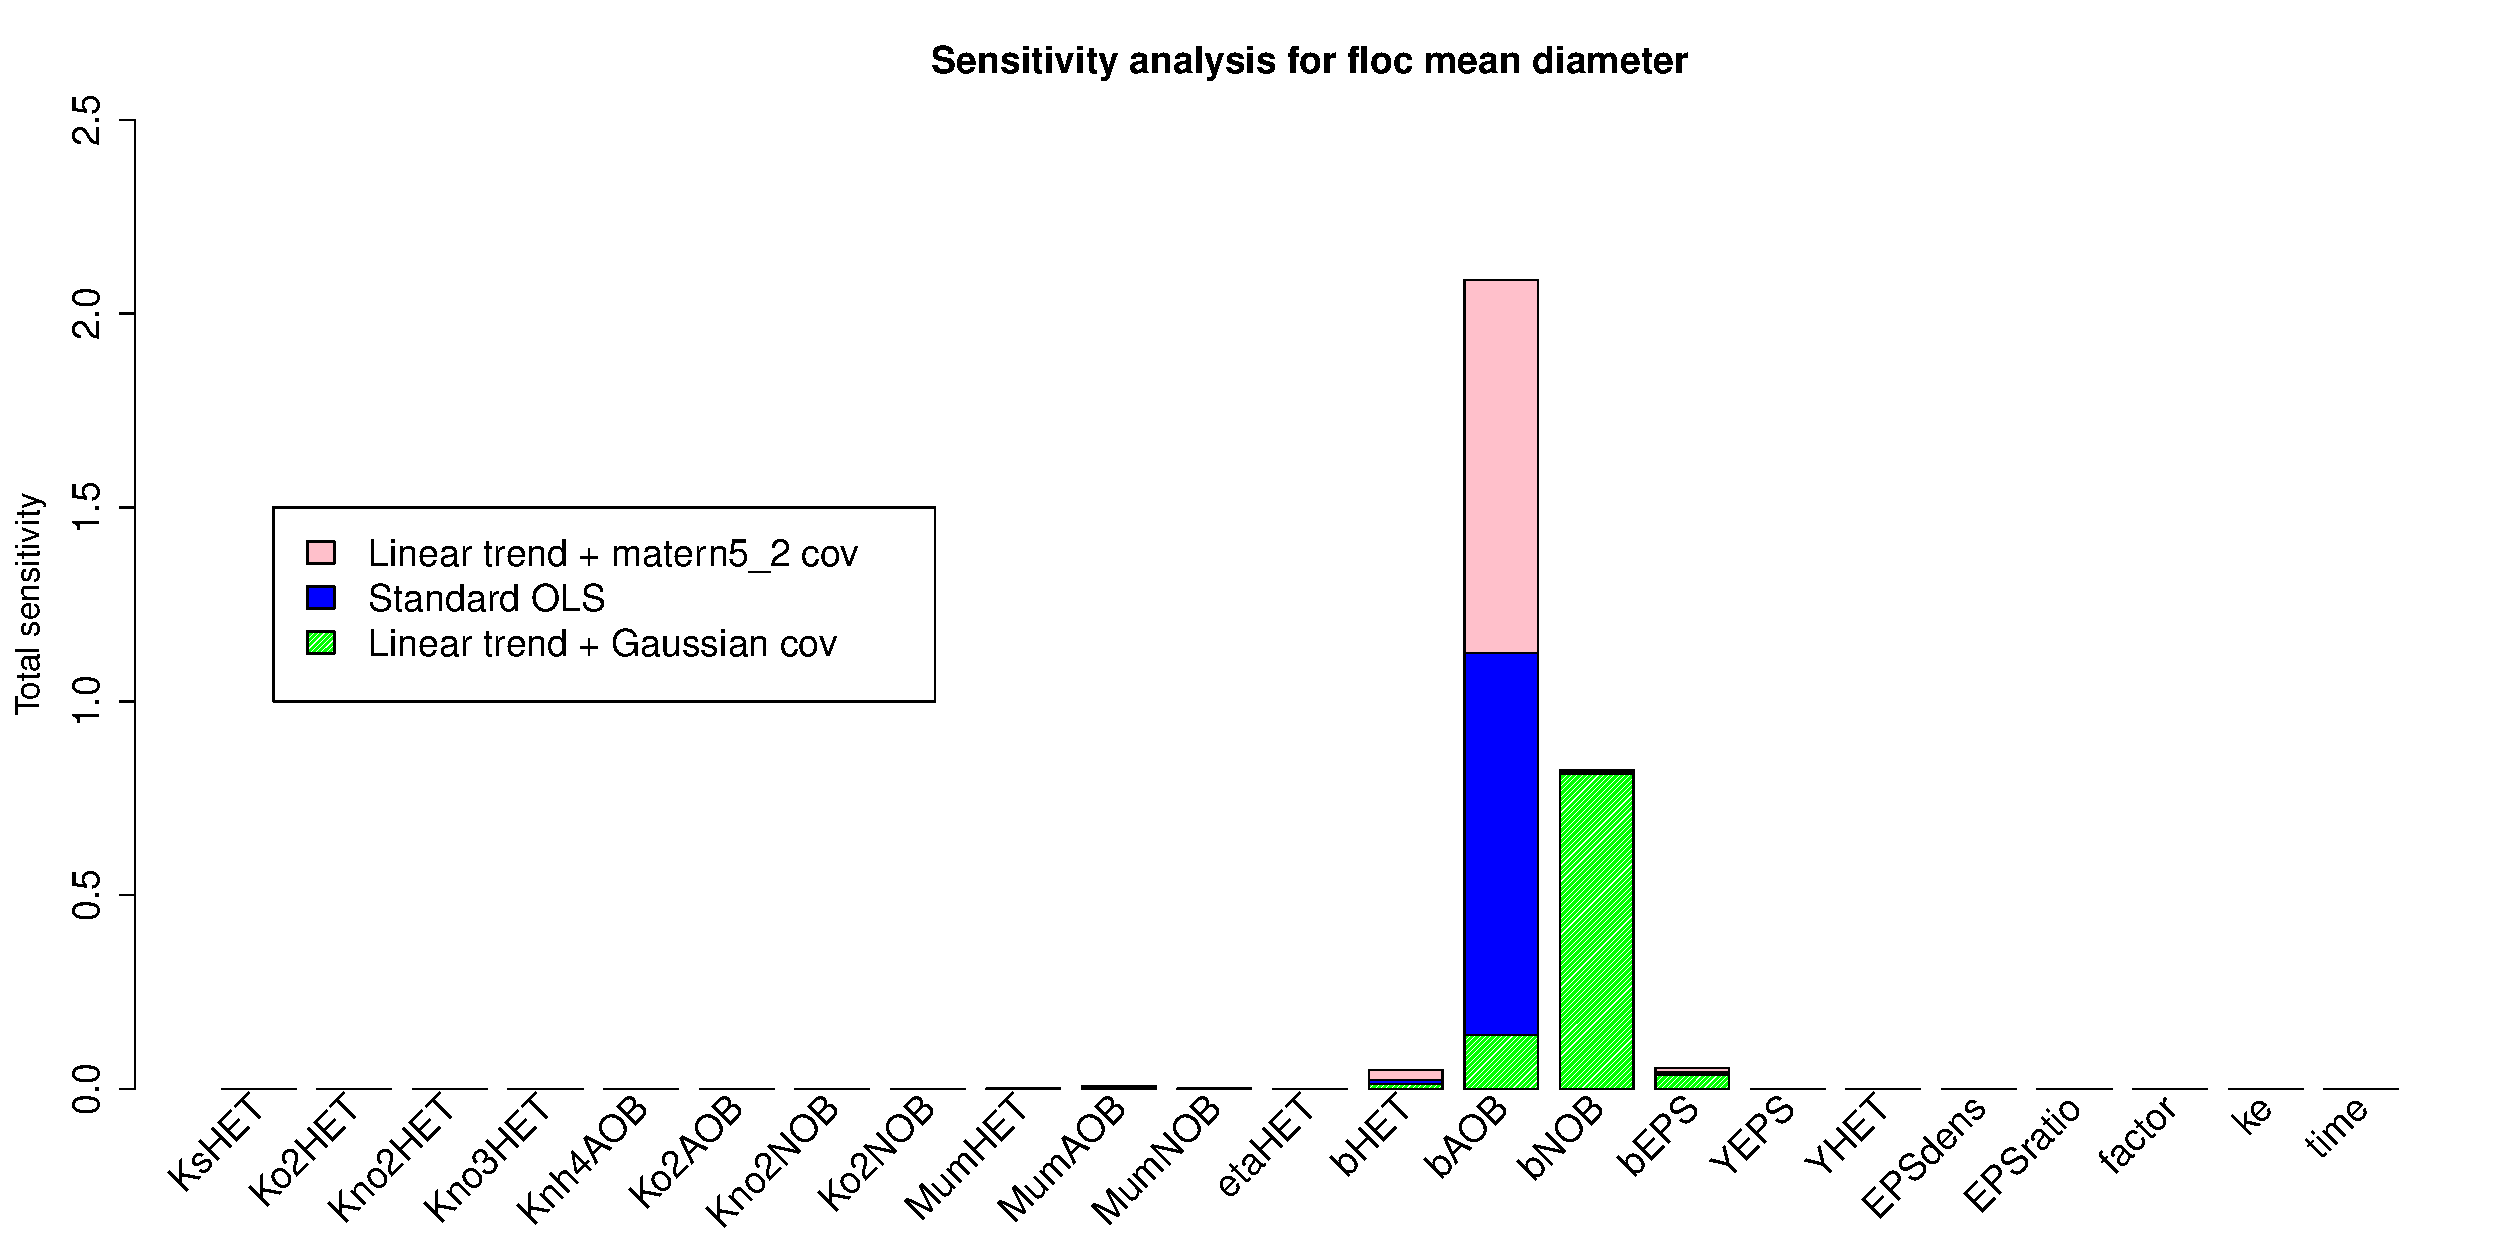
\includegraphics[width=1.1\textwidth]{ana/sensitivty_results}
\caption[]{Barplots showing total sensitivity indices for mean floc diameter using Sobol based variance decomposition technique. Comparison for three different methods.}\label{sens}
\end{figure}

%problems of optimization (cost of objective functions, numerical instabilities, multimodality and dimensionality issues)
%%%%%%
%for the fast and efficient estimation of trend and covariance parameters relying on a global optimizer with a gradient like the genoud algorithm of the package $rgenoud$
%assumed to be constructed by stepwise technique.
%Noninformative Bayesian analysis leads to kriging predictor and variance 
%appear respectively as conditional mean and variance, and the analytically tractable conditional covariance kernel enables the use of conditional simulations at any set of new design points.
%\chapter*{Appendix}

\chapter{Emulation of floc and biofilm}
\section{Introduction}
 Flocs are aggregation of microbes mixed with an adhesive material called EPS. They are often difficult to measure or quantify because of their irregular size and shape.  A wide range of different equivalent diameters is often used to characterize the floc size, see \citet{l3} for further details. The individual particle that makes up the flocs are simulated as a sphere of a variable volume. 
Our approach is to focus on the cluster of particles as a floc because of a large number of data involve and emulate their interested properties stated below.  The floc is treated as a ball of a sphere, and we estimate the diameter of a sphere that circumscribes its boundary/outline. The center of the sphere will be equivalent to the center of mass of the component particles as shown Figure (\ref{diag2}). The detailed procedure of emulating the floc diameter and (biofilm) will be described in this section. In the further analysis, we will also emulate the center of the sphere to give spatial attributes to the floc characterization.

\section{Simulation}
Let the design matrix which contain the input to the LAMMPS model be denoted by $\bX=(\theta^i_p, t, p=1,\ldots,25; i=1,\ldots,1000)$, where the subscript $p=25$ represents 20 callibrated model parameters and 5 variables that represent the model initial conditions (see Table \ref{mytab1}), superscript $i$ denote the 1000 different realisations (design points) and $t$ is the time slice in seconds at which the output data is recorded $t=1,\ldots,T$. The design matrix $\bX_{1000 \times 26}$ denotes the input values at which the LAMMPS model is run for every combinations of $x_i$ which is a point in $\bX$, where $x_i$ represents $i^{th}$ row of $\bX$.  The LAMMPS code is run for two days (~172800 s simulation time). 

The simulations are repeated 100 times at each design point $i$ to incorporate stochastic variations in our outputs and are recorded at a time-step of 2000 seconds which gives about 86 different time slices. This will provide initial estimates of the mean and variance of the LAMMPS model.

The current LAMMPS code is set up to produce the following outputs namely particle diameter, mass, position (3-dimensional) for each time step $t$. The time series output at each design point is denoted as a matrix $\bY=[\by_1,\ldots,\by_T]$, such that $\by=[y_1,\ldots,y_n]$,  where $T=86$ in this simulation and $n$ is the total number of particles at each time step. The number of particles $n$ at each time slice varies across the design points and, in particular, increasing with time as it expected for the microbes to be growing. An independent simulation of 100 runs with ten replicates is performed for cross-validation purpose. Here, the simulation is run for a longer period than the previous simulations (~4 days simulation). 
We consider emulation of floc which is summarized by aggregating all the individual microbe at each time step. 

\section{Procedure for emulating floc equivalent diameter}
\begin{figure}[!ht] 
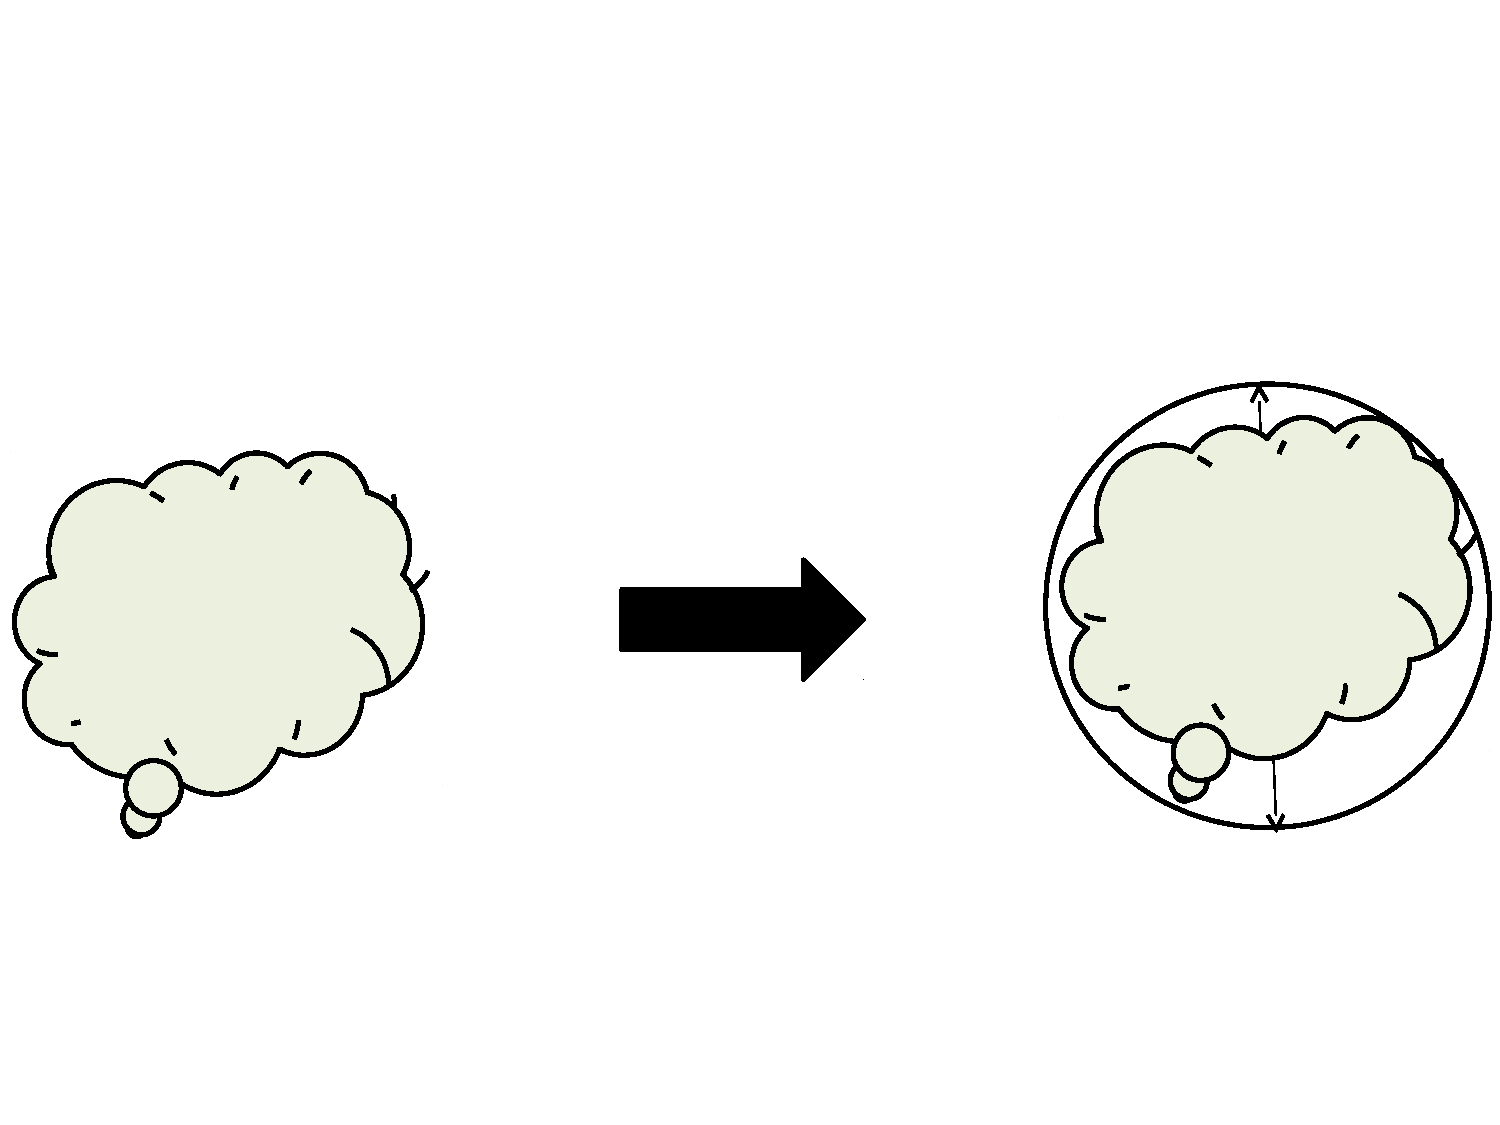
\includegraphics[width=1.1\textwidth]{diagram2}
\caption[]{Transformation of microscale particles to floc at the mesoscale. Floc equivalent diameter is the diameter of the smallest sphere that circumscribes the outline of the projected floc.}\label{diag2}
\end{figure}

\section{The challenges}
Some of the major challenges of LAMMPS emulation are the nature of the outputs produced from the model that make it much difficult to emulate
\begin{itemize}
\item[(1)] The LAMMPS model is expensive to evaluate - we can not run it at every parameter combination of interest, which limits the amount of information we have 
\item[(2)] The LAMMPS model is stochastic in nature - this introduces much randomness in the data
\item[(3)] The model produces high-dimensional and multiple outputs which make the emulation more computationally demanding than usual
\item[(4)] The LAMMPS model is dynamic
\end{itemize}
Despite all these caveats, the good news is that there is a large knowledge base addressing these problems.
There is a limited number of literature that treat emulation of stochastic simulators. Earlier work of \citet{pd23} performs ordinary kriging emulation of detrended and standardized response $\by'$ from stochastic outputs. 
The scale response is derived by repeating the simulation $k$ times at each design point such that
$\by'=\frac{\bar \by-\hat  f}{\mathbf{\sigma}^2/\sqrt{k}}$, where $\bar \by(x_i)=\frac{\sum_{j=1}^k\by_{ij}}{k}$, $\sigma^2(x_i)=\frac{\sum_{j=1}^{k}(\by_{ij}-\bar \by)^2}{k-1}$ and $\hat  f$ is estimate of main signal function. This approach was extended by \citet{pd24} where an independent GP emulator is developed for both the mean response and stochastic (noise) variance.  A related approach was documented in \citet{pd22} and \citet{pd25} where an additional GP model is built to estimate the noise variance of the noise-free dataset.
In addition to developing a model for the mean response, \citet{pd21} also fit empirical log-transformed noise variance in an heteroscedastic GP modelling of a stochastic simulator.  Similar to \citet{pd24,pd21}, \citet{pd26} focuses on the emulation and calibration of a stochastic computer model, implementing two independent Gaussian processes on the sample mean and log-transformed standard deviation of simulation outputs. The independent GP models use a nugget parameters to account for sampling error in the data. 

Our initial treatment of the stochasticity in the model is to perform multiple runs and average the key outputs which are then taken as deterministic in nature. The second approach is to incorporate nugget terms in form empirical variance derived from the sampling data.

\subsection{Dynamic emulator}
Due to the nature of output data from LAMMPS model, we consider using a dynamic emulation technique. Dynamic emulation models the evolution or trajectory of random variables over some
time-steps \citep{pd12}. Emulation of time-series data or physical processes that evolve with time which implies that model output at time $t$ becomes an input to the model at time $t+1$. The model can be written as 
\begin{equation}\label{dyna3}
\by_t = f(\bx_t, \by_{t-1})
\end{equation}
Where $\by_{t-1}$ is the state vector at the previous time step for $t={1,\ldots,T}$, and $\bx_t$ are the inputs at time $t$ which includes the model parameters, forcing and initial conditions. There are two fundamental techniques for addressing dynamic emulation as discussed in \citep{pd12}. The multi-step and single-step emulations and there are about three different variants of the multi-step technique.


\subsection{Multi-step emulation}
Firstly, we can emulate a complete multi-step run of the computer model. One of the ways to proceed with this according to \citet{pd14} is to treat the problem as a multivariate output simulator and develop a multi-output emulator where the dimension of the output space is given as $T$. Closely related to this approach, is to build one single-output emulator that incorporates time as an additional input to the emulator such that $\by_t = f(\bx,t)$, where the training data for building emulator consists $nT$ data points. The problem with this approach is that it is not efficient in practice because the dimension of the data becomes vast which introduces additional computational difficulty. 

The third variant is to emulate each time step, which produces an emulator that is specific to a particular time step, an approach that assumes independence between the time steps. This method was used in \citet{pd27} but is not suitable for our present data. Here, where are interested in the temporal correlations across the time steps, and specifically for using an emulator to scale up LAMMPS model outputs from an order of O($10^6$) particles to O($10^{13}$) particles, i.e., for making multiple-step ahead predictions.

\subsection{Single-step emulation}
The second method is to model the simpler, single step simulator and use the emulator recursively to generate the full-time series of the resulting predictions up to the number of desired time points. This reduces the dimension of the problem. We implemented both methods for emulation floc equivalent diameter. Although, the single-step emulation seems much appealing for our upscaling problem considering fact that we want to capture the complete behaviour of floc diameter over a number of time steps.

%\subsubsection{Iterative (single-step) emulation}
We describe the single step function emulation here. We follow a similar procedure described in \citet{pd12} and \citet{pd17}. Starting from initial run of the model at time $t_0$, we construct the single step emulator $\by_1 = f(\bx_1, \by_{0})$ using  a GP regression in form of kriging. One of the usefulness of dynamic emulation is to make a multiple step ahead predictions using iterative technique to repeat one-step-ahead predictions until the desired number of points. We proceed sequentially, feeding back the entire output distribution from the GP model, such that at time step $t=1$, for input $(\bx_1,\by_0)$, the model output is given as $$\tby_1 \sim N(\hby(x_1,y_0), \hat S^2(x_1,y_0)).$$
For the next prediction at time $t=2$, the input data $\bx_2$ is augmented by complete distribution $\by^{(i)}_1$ such that $\bX_2=[(\bx_2,\tby_1)]^T$, then we have $$\tby_2 \sim N(\hby(x_2,\tby_1), \hat S^2(x_2,\tby_1)).$$ This procedure is repeated until $T-1$ steps is reached.

The construction of single-step emulator is summarized below:
\begin{itemize}
 \item[{(i)}] Subsample 300 points randomly from original 1000 points and formulate a single step emulator using equation (\ref{dyna3}) such that $\by_1=f(\bx,\by_0)$, where $\bx$ is the new design matrix for running the LAMMPS model for the single step function, $\bx$, as usual, includes previous value of the state variable $\by_{0}$, initial conditions and calibrated (constant) parameters while the corresponding output is the value of current state variable $\by_t$.

\item[{(ii)}] Perform the GP emulation in the form of kriging as described in previous chapter 2, where we use a quadratic mean and exponential covariance functions. Parameters $\theta=[\hbbeta, \hat{\sigma^2},\bhalpha]$ are estimated by MLE technique.

\item[{(iii)}] Compute the posterior distribution of $p((.)|\by,\hat\theta)\sim N(\hby(x_0), \hat S^2(x_0))$ where $\hby(x)$ and $\hat S^2(x)$ are defined in equations (\ref{man}, \ref{olu2b}) respectively.

\item[{(iv)}] Use the emulator to simulate from $p((.)|\by_1,\hat\theta)$  to obtain $\tby_{1}$ and then iterate the next steps for $t=1,\ldots,T-1$ to give a full time series $[\tby_1,\ldots,\tby_{T-1}]$. 

\item[{(v)}] Derive a new training data by augmenting the original data by simulated time series and rebuild the single-step emulator with the new training data given below. 
\[ 
\left( \begin{array}{ccc}
\mbox{Original inputs}\\
~\vdots \\
(\by_0,\bx_1)\\
(\tby_1,\bx_2)\\
~~\vdots \\
(\tby_{T-1},\bx_T) \end{array} \right)
 = 
\left( \begin{array}{ccc}
\mbox{Original outputs}\\
~\vdots \\
\tby_1\\
\tby_2 \\
~\vdots \\
\tby_{T}\end{array} \right).
\] 
\item[{(vi)}] Simulate $\tby_{t+1}$ from conditional distribution $p((.)|\by_t,\hat\theta)$  
\item[{(vii)}] Repeat the entire process many times to obtain $\tbY^{N}=[\tby_1,\ldots,\tby_{T-1}]^N$, where
$\tbY^{N}$ is a sample from the joint distribution of $[\by_1,\ldots,\by_{T-1}]$ given the emulator training data and initial conditions and $N$ is the number of Monte Carlo (MC) sample.
\end{itemize}


\section{Results}
Suppose at time step $t$, the LAMMPS output is written in the form 
\begin{equation}
\by_t=f(\bx_t,\by_{t-1})
\end{equation}
Where $\by_{t-1}$ the state vector at the previous time step, $\bx_t$ are the input at time $t$ which includes the model parameters, forcing and initial conditions as described earlier. We summarize the indiviudual particle at microscale to a large (mesoscale) as a floc. We consider emulation of floc which is summarized by aggregating all the individual microbe at each time step. The number of particles $n$ at each time slice varies across the design points as stated before. The number of design points at each time step is $1000$ and $T=86$ in our simulation. The total floc mass at time $t$ is given as
\begin{equation}
M_t =\sum^n_{k=1} m_{kt},
\end{equation} 
and center of mass $\tC$ for the floc aggregate in 3-dimension, for $X$ direction using equation 
\begin{equation}\label{com}
\tP_{x_t}=\frac{\sum^n_{k=1} m_{kt} X_{kt}}{M_t},
\end{equation}
where $M_t$ is the total floc mass at time $t$ for all the species and $m_{kt}$'s are individual particle level mass. Replace $X_{kt}$ in equation (\ref{com}) with $Y_{kt}$ and $X_{kt}$ respectively to derive for other directions.

 There are two different ways to derive the floc equivalent diameter namely the volume and distance techniques. Under the distance approach, the diameter of the smallest circle that circumscribes the outer edge or sketch of the floc can be obtained by computing relative distances in $X-Y-Z$ positions of each of the particle from the center of mass of the floc aggregate. The sum of the maximum of this distances and radius of the particle with the largest distance will form the radius of the outer sphere as shown in Figure (\ref{diag2}). 

Suppose at time $t$, the distance in euclidean three-space between any two positions, say particle $p$ at position $P=(x_k,y_k,z_k)$ and floc center of mass at point $\tP=(x_0,y_0,z_0)$ is given as
%\begin{equation}
 $d_{k}=\sqrt{(x_{kt}-x_0)^2+(y_{kt}-y_0)^2+(z_{kt}-z_0)^2}, $
%\end{equation}
\begin{equation}
d_{eqv}=2(\max{(d_{k})}+r_{k'}) ,
\end{equation}
where $r_{k'}$ is the radius of particle with largest distance and $x$, $y$ and $z$ are respective directions, $k=1,\ldots,n$. 
The second approach is to compute the total volume of the floc using the volume of each individual particle (particle is taken as a sphere).
\begin{equation}
d_{eqv}=\sum^n_{k=1} \sqrt[3]{\frac{6V_{kt}}{\pi}}
\end{equation}
where $V_{kt}$ volume of individual spherical particle $k$ at time $t$, $\pi$ is a constant and $d_{eqv}$ is the floc equivalent diameter. The volume technique under-estimates the value of equivalent diameter.

% These input points reasonably fill the design space as is important to exploring the global characteristics of the simulator. the nugget matrix based on sample variances for replicate design points (which is easily obtained using the

\begin{itemize}
\item[(i)] Biofilm /floc total mass at each time step
\item[(ii)] Biofilm /floc equivalent diameter at each time step
\item[(iii)] EPS total mass at each time step
\item[(iv)] Total number of particles at each time step
\item[(v)] The mass ratio of individual particle to the total biofilm /floc mass
\item[(vi)] Distribution of floc/ biofilm diameter
\item[(vii*)] Change in the nutrient environment of the floc (defer until the chemistry and hydrodynamics are coupled to the model).
%\item[(viii*)] Biofilm surface enlargement (still tricky; need to liaise with Prashant/Jaya)
\end{itemize}

%Wastewater treatment plant optimization focuses on aggregate outcomes of individual particle-level processes and behavioural rules. 


%We describe the single step emulation procedure which involves iteratively or recursively modelling the state variable such that
%\begin{equation}
%y_t = f(x_t , y_{t-1}) = f (x_t , f(x_{t-1}, y_{t-2})    )
%\end{equation}
%$$= f (x_t , f(x_{t-1},\ldots,f(x_1, y_0))    )= f^{(t)} (x, y_0)$$, such that $f^{(t)}(.)$ is a $t$ step simulator with input parameters $x$ and $y_0$ is the initial state vector of the simulation, $t=1,\ldots,p$.

%The number of design points at each time step is denoted as $n=1000$ and $T=86$ in our simulation.

\chapter{Biofilm emulation}

\begin{figure}[!ht] 
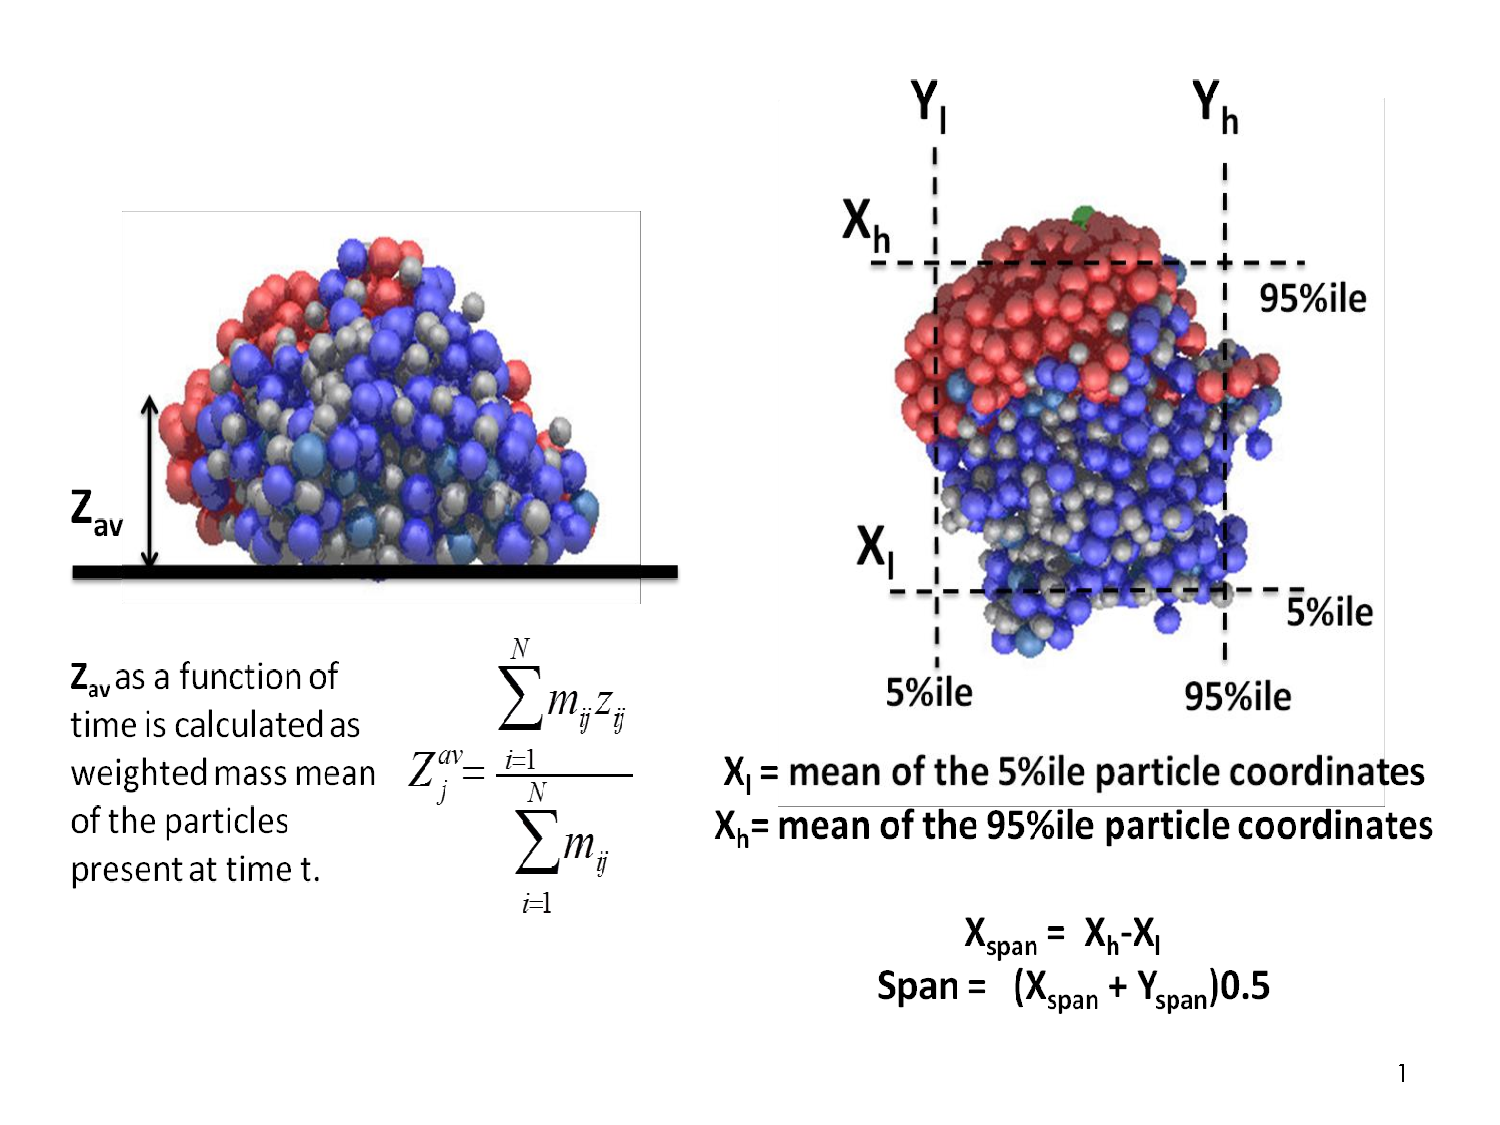
\includegraphics[width=1.1\textwidth]{result2/bio_char}
\caption[]{Biofilm characterization}\label{diag22}
\end{figure}


\begin{thebibliography}{94}
%\cleardoublepage
%\phantomsection
\bibliographystyle{plain}

\bibitem[Currin et al.(1991)]{pd1} Currin, C., Mitchell, T.J., Morris, M.D., and Ylvisaker, D. (1991). Bayesian Prediction of Deterministic Functions, With Applications to the Design and Analysis of Computer Experiments. {\it Journal of the American Statistical Association}, $86(416), 953-963$. 

\bibitem[Martin \& Simpson(2004)]{pd2} Martin, J. D., \& Simpson, T. W. (2004). On the use of kriging models to approximate deterministic computer models. {\it In ASME 2004 International Design Engineering Technical Conferences and Computers and Information in Engineering Conference}, $481-492$.

\bibitem[Osio et al.(1996)]{pd3} Osio, I.G. and Amon, C.H. (1996). An Engineering Design Methodology with Multistage Bayesian Surrogate and Optimal Sampling. {\it Research in Engineering Design}, $8(4), 189-206$.

\bibitem[Sacks et al.(1989)]{pd4} Sacks, J., Welch, W., Mitchell, T., Wynn, H. (1998). Design and analysis of computer experiments. {\it Statistical Science}, $4(4), 409-435$.

\bibitem[Santner et al.(2003)]{pd5} Santner, T., Williams, B., Notz, W. (2003). The Design and Analysis of Computer Experiments. Springer.

\bibitem[Li \& Sudjianto(2005)]{pd6} Li, R., \& Sudjianto, A. (2005). Analysis of computer experiments using penalized likelihood in gaussian kriging models. {\it Technometrics}, $47(2), 111-120$.

\bibitem[Andrianakis \& Challenor(2009)]{pd7} Andrianakis, Y., \& Challenor, P. G. (2009). Parameter estimation and prediction using gaussian processes. {\it Technical report}, MUCM Technical report 09/05, University of Southampton.

\bibitem[Roustant et al.(2012)]{pd8} Roustant, O., Ginsbourger, D., \& Deville, Y. (2012). DiceKriging, DiceOptim: Two R packages for the analysis of computer experiments by kriging-based metamodeling and optimization.

\bibitem[Park \& Baek(2001)]{pd9} Park J.S., \& Baek, J. (2001). Efficient Computation of Maximum Likelihood Estimators in a
Spatial Linear Model with Power Exponential Covariogram. {\it Computer Geosciences}, $27, 1-7$.

\bibitem[Hankin(2005)]{pd10} Hankin, R. K. (2005). Introducing BACCO, an R package for Bayesian analysis of computer code output. {\it Journal of Statistical Software}, $14, 16$.

\bibitem[O'Hagan(2006)]{pd11} O'Hagan, A. (2006). Bayesian Analysis of Computer Code Outputs: A Tutorial. {\it Reliability Engineering and System Safety}, $91, 1290-1300$.

\bibitem[Conti et al.(2009)]{pd12} Conti, S., Gosling, J. P., Oakley, J. E., \& O'hagan, A. (2009). Gaussian process emulation of dynamic computer codes. {\it Biometrika}, asp028.

\bibitem[Conti et al.(2004)]{pd13} Conti, S., Anderson, C. W., Kennedy, M. C., \& O’Hagan, A. (2004). A Bayesian analysis of complex dynamic computer models. {\it In Proc. of the 4th International Conference on Sensitivity Analysis of Model Output}.

\bibitem[Conti et al.(2010)]{pd14} Conti, S., \& O’Hagan, A. (2010). Bayesian emulation of complex multi-output and dynamic computer models. {\it Journal of statistical planning and inference}, $140(3), 640-651$.

\bibitem[Bhattacharya(2007)]{pd15} Bhattacharya, S. (2007). A simulation approach to Bayesian emulation of complex dynamic computer models. {i\t Bayesian Analysis}, $2(4), 783-815$.

\bibitem[Kennedy et al.(2001)]{pd16} Kennedy, M.C., \& O'Hagan, A. (2001). Bayesian calibration of computer models. {\it Journal of the Royal Statistical Society}. Series B, Statistical Methodology, $425-464$.

\bibitem[Azman \& Kocijan (2005)]{pd17} Azman, K., \& Kocijan, J. (2005). Comprising prior knowledge in dynamic gaussian process models. {\it In Proceedings of the International Conference on Computer Systems and Technologies-CompSysTech}, Vol. 16(17.6).

\bibitem[Kleijnen(2009)]{pd18} Kleijnen, J. P. (2009). Kriging metamodeling in simulation: A review. {\it European Journal of Operational Research}, $192(3), 707-716$.

\bibitem[Kleijnen \& Simpson(2005)]{pd19} Martin, J. D., \& Simpson, T. W. (2005). Use of kriging models to approximate deterministic computer models. {\it AIAA journal}, $43(4), 853-863$.

\bibitem[Kleijnen \& Mehdad(2014)]{pd20} Kleijnen, J. P., \& Mehdad, E. (2014). Multivariate versus univariate kriging metamodels for multi-response simulation models. {\it European Journal of Operational Research}, $236(2), 573-582$.

\bibitem[Boukouvalas et al.(2009)]{pd21} Kleijnen, J. P. (2009) Boukouvalas, A., Cornford, D., \& Singer, A. (2009). Managing uncertainty in complex stochastic models: {\it Design and emulation of a rabies model. In 6th St. Petersburg Workshop on Simulation}, (pp. 839-841).

\bibitem[Kersting et al.(2007)]{pd22} Kersting, K., Plagemann, C., Pfaff, P., \& Burgard, W. (2007). Most likely heteroscedastic Gaussian process regression. {\it In Proceedings of the 24th international conference on Machine learning}, (pp. 393-400). ACM.

\bibitem[Kleijnen \& Beers(2005)]{pd23} Kleijnen, J.P., \& Van Beers, W.C. (2005). Robustness of kriging when interpolating in random simulation with heterogeneous variances: Some experiments. {\it European Journal of Operational Research}, $165(3), 826-834$.

\bibitem[Bates et al.(2006)]{pd24} Bates, R. A., Kenett, R. S., Steinberg, D. M., \& Wynn, H. P. (2006). Achieving robust design from computer simulations. {\it Quality Technology and Quantitative Management}, $3(2), 161-177$.

\bibitem[Bates et al.(1997)]{pd25} Goldberg, P. W., Williams, C. K., \& Bishop, C. M. (1997). Regression with input-dependent noise: A Gaussian process treatment. {\it Advances in neural information processing systems}, $10, 493-499$.

\bibitem[Henderson et al.(2012)]{pd26} Henderson, D. A., Boys, R. J., Krishnan, K. J., Lawless, C., \& Wilkinson, D. J. (2012). Bayesian emulation and calibration of a stochastic computer model of mitochondrial DNA deletions in substantia nigra neurons. {\it Journal of the American Statistical Association}.

\bibitem[Boukouvalas et al.(2014)]{pd27} Boukouvalas, A., Sykes, P., Cornford, D., \& Maruri-Aguilar, H. (2014). Bayesian precalibration of a large stochastic microsimulation model. {\it Intelligent Transportation Systems, IEEE Transactions on}, $15(3), 1337-1347$.

\bibitem[Kleijnen \& Mehdad(2012)]{pd28} Kleijnen, J., \& Mehdad, E. (2012). Kriging in multi-response simulation, including a Monte Carlo laboratory. {CentER Discussion Papers Series}, (2012-039).


\bibitem[Jarvis et al.(2005)]{l3} Jarvis, P., Jefferson, B., \& Parsons, S. A. (2005). Measuring floc structural characteristics. {\it Reviews in Environmental Science and Bio/Technology}, $4(1-2), 1-18$.

\end{thebibliography}{}

\section*{Appendix 1: Estimation of prior hyperparameters}\label{hyper}
Noting that under GP regression, the prior distribution for the data is also a Gaussian distribution, the joint likelihood of the parameters is given as
\begin{equation}\tag{A.10}\label{like}
p(\boldsymbol \beta, \sigma^2, \boldsymbol{\alpha}|\by)\propto \frac{det(\bf C)^{-\frac{1}{2}}}{{(2\pi\sigma^2)}^\frac{n}{2}}\exp \Big \{\frac{(y-H\boldsymbol \beta)^T \bf C^{-1}(\by-H\boldsymbol \beta)}{2\sigma^2}\Big\}
\end{equation}
where $\boldsymbol{\alpha}=[\alpha_1, \ldots, \alpha_n]$ is a vector of correlation lengths and $det(\bf C)$ is the determinant of correlation matrix $\bf C$, integrating out $\boldsymbol \beta$ using a non-informative (uniform) prior such that $p(\boldsymbol \beta) \propto$ 1. We have a marginal likelihood
\begin{equation}\tag{A.10b}\label{like2}
p(\by|\sigma^2, \boldsymbol{\alpha})\propto \frac{\det(\bf C)^{-\frac{1}{2}}\det(H^TCH)^{-\frac{1}{2}}}{{(2\pi\sigma^2)}^\frac{n-p}{2}}\exp \Big \{\frac{(\by-\bH\hbbeta)^T \bC^{-1}(\by-\bH\hbbeta)}{2\sigma^2}\Big\}.
\end{equation}
Maximizing (\ref{like2}) with respect to $\boldsymbol \beta$ and $\sigma^2$ will give %the MLE of $\boldsymbol \beta$ 
\begin{equation}\tag{A.11}
\hbbeta=(\bH^T\bC^{-1}\bH)^{-1}\bH^T\bC^{-1}\by
%(\ref{like3})
\end{equation}

\begin{equation}\tag{A.12}
\widehat{\sigma^2}=\frac{1}{n-p}\Big[\mathbf{(y-H\hat{\boldsymbol \beta})}^T\bf C^{-1}(\bf y-H\hat{\boldsymbol \beta})\Big]
\end{equation}
Now, integrate out $\sigma^2$ such that $p(\sigma^2) \propto \frac{1}{\sigma^2}$, then we have
\begin{equation}\tag{A.10c}\label{like3}
p(\by|\boldsymbol{\alpha})\propto \det(\bC)^{-\frac{1}{2}}\det(\bH^T\bC\bH)^{-\frac{1}{2}} \Big \{(\by-\bH\hbbeta)^T \bC^{-1}(\by-\bH\hbbeta)\Big\}^{-(n-p)/2}
\end{equation}
$$=\det(\bC)^{-\frac{1}{2}}\det(\bH^T\bC\bH)^{-\frac{1}{2}} {\widehat{\sigma^2}}^{-(n-p)/2}.$$
%The smoothing parameter $\boldsymbol{\alpha}$ is estimated by maximizing the marginal likelihood (\ref{like3}) using the posterior mode%, the estimates of $\hat{\boldsymbol \beta}$ and $\widehat{\sigma^2}$ are substituted in equation (\ref{like}) and maximized over $\boldsymbol \beta$ and $\sigma^2$ to obtain


The smoothing parameter $\boldsymbol{\alpha}$ is estimated from the posterior distribution using the posterior mode by the value of $\boldsymbol{\alpha}$ for which marginal likelihood (\ref{like3}) is maximised. Here, we describe briefly the maximisation of the posterior distribution of $\boldsymbol{\alpha}$ which is reparametrized as $\btau=2log(\boldsymbol{\alpha})$ to make it unconstrained optimisation \citep{pd7, pd5}. 
Therefore, function $f(\btau)=log(p(\by|\exp(\frac{\btau}{2})))$ can be optimised using a derivative-free numerical optimisation of Nelder-Mead method which is the default in the "emulator" package that we use.
%\begin{equation}\tag{A.13}
%L(\hat{\boldsymbol \beta},\widehat{\sigma^2},\boldsymbol{\alpha})=-\frac{1}{2}\Big[n~log(\widehat{\sigma^2})(\boldsymbol{\alpha})+log(det(\bf C(\boldsymbol{\alpha})))+\textnormal n\Big],
%\end{equation}
%which is a function of $\boldsymbol{\alpha}$ that can be computed using a derivative-free numerical optimisation like Nelder-Mead method see further details in %\citep{70,q10}.
%Posterior distribution is obtained as $P(\mathbf{z}|\widehat{\boldsymbol\beta},\hat\sigma^2,\hat\alpha)\sim N[m^{\bullet}(u),\sigma^2C^{\bullet}(u,u')]$, with posterior mean and covariance functions given as equations (\ref{olu1} and \ref{olu2}) respectively.

\begin{table}
\caption{List of LAMMPS model parameters}\label{mytab1}
\centering
\fbox{
\begin{tabular}{*{2}{c|c|c}}
Index&List of parameters& Value\\ 
\hline \hline
1&KsHET &0.01\\
2&Ko2HET & 0.81\\
3&Kno2HET & 0.0003\\
4&Kno3HET & 0.0003\\

5&Knh4AOB & 0.001\\
6& Ko2AOB & 0.0005\\

7&Kno2NOB & 0.0013\\
8&Ko2NOB & 0.00068\\
\hline
&Defining maximum growth variables\\
\hline
9&MumHET & 0.00006944444\\
10&MumAOB & 0.00003472222\\
11&MumNOB & 0.00003472222\\
12&etaHET & 0.6\\
\hline
&Defining decay rates variables\\
\hline 
13& bHET & 0.00000462962\\
%#variable bHET & 0.00462962\\
14&bAOB & 0.00000127314\\
%#variable bAOB & 0.00127314\\
15&bNOB & 0.00000127314\\
%#variable bNOB & 0.00127314\\
16&bEPS & 0.00000196759\\

17&YEPS & 0.18\\
18&YHET & 0.61\\
%19&variable EPSdens & 30\\
19&EPSratio & 1.25\\
20&factor & 1.5\\
\hline
&Initial conditions (nutrients)\\
\hline
21&sub &0.08 \\
22&no2 & 0.008\\
23&no3 & 1e-05\\
24&o2 & 0.01\\
25&nh4 &0.09\\
%22&variable ke & 5e+10
\end{tabular}}
\end{table}

\end{document}
